%! Unidad 8 — Principios básicos de cinemática (teoría, ejemplos resueltos, ejercicios por apartados, lectura, prácticas y situación de aprendizaje)
%! Fuente: Fuentes/Fisica/Unidad 8 (capturas 186-200 y solucionario). Texto reescrito; datos de los ejercicios cambiados y recalculados.
%! Notación: vectores unitarios \ivec, \jvec, \kvec y la «d» de las derivadas \dif (definidos en el principal).
%! Figuras en images/UD8/: nuevas en html/ (sistemas_referencia, velocidad_limite, velocidad_relativa, aceleracion_media,
%!   componentes_intrinsecas, aerodeslizador) y copiadas (PDF + SVG) de 4ESO/images/UD7 (posicion_trayectoria,
%!   tipos_trayectoria, velocidad_vector). Gráficas de trayectorias con pgfplots (estilo «grafica» del principal).

\section*{Para empezar: ¿quién se mueve en el telesilla?}
\addcontentsline{toc}{section}{Para empezar: ¿quién se mueve en el telesilla?}

Imagina que estás en una estación de esquí, esperando en la cola del telesilla. Mira a tu alrededor: ¿se mueven los árboles, las
farolas o la caseta de los remontes? Está claro que no. Unos minutos después ya vas sentado en el telesilla, subiendo hacia la
cumbre junto a una amiga. Hazte ahora las mismas preguntas: los árboles y las farolas pasan a tu lado y van quedando atrás, mientras
que tu amiga, que hace un momento se movía hacia ti por la cola, sigue siempre a tu lado, \textbf{en reposo respecto a ti}.

Las respuestas han cambiado porque ha cambiado el punto desde el que observas. El \textbf{movimiento} y el \textbf{reposo} no son
absolutos: dependen del observador. En las pistas, los esquiadores, los telesillas o los telecabinas describen trayectorias rectas y
curvas, aceleran, frenan y giran. En esta unidad aprenderemos a describir esos movimientos con precisión mediante vectores y
derivadas, sin preocuparnos todavía de las causas que los producen, que estudiaremos en las unidades de dinámica.

%========================================================================================
\section{Recuerda de la ESO}\label{sec:ud8-eso}
%========================================================================================

\paragraph{Magnitudes escalares y vectoriales.} Una magnitud es \textbf{escalar} si queda definida con un número y su unidad: la
masa, el tiempo, la temperatura o la distancia de tu casa al instituto (\qty{800}{\m}). Es \textbf{vectorial} si además hay que
indicar una \textbf{dirección} y un \textbf{sentido}: decir que un coche va a \qty{110}{\km\per\hour} no basta para saber dónde
estará dentro de una hora; hay que añadir por qué carretera va y hacia dónde. Las magnitudes vectoriales se representan con
\textbf{vectores}, flechas con módulo, dirección y sentido.

\paragraph{El movimiento.} Un cuerpo se mueve si su posición cambia con el tiempo respecto a otro cuerpo que tomamos como
referencia. Mientras lees, estás en reposo respecto a tu silla, pero te mueves a gran velocidad respecto al Sol: el movimiento es
\textbf{relativo}.

\paragraph{Trayectoria y desplazamiento.} La \textbf{trayectoria} es el camino que sigue el cuerpo; según su forma, el movimiento
es \textbf{rectilíneo} o \textbf{curvilíneo}. El \textbf{desplazamiento} es la distancia en línea recta entre las posiciones
inicial y final, y el \textbf{espacio recorrido}, la distancia medida sobre la trayectoria. Solo coinciden si la trayectoria es
recta y el cuerpo no cambia de sentido. En una trayectoria cerrada (una vuelta a la pista) el desplazamiento es nulo, pero el
espacio recorrido no.

\paragraph{Velocidad y aceleración.} La \textbf{velocidad} mide lo deprisa que cambia la posición de un cuerpo, y la
\textbf{aceleración}, lo deprisa que cambia su velocidad. En el SI se miden en \unit{\m\per\s} y en \unit{\m\per\s\squared}.

\paragraph{Cambios de unidades.} Las magnitudes fundamentales de la cinemática son la \textbf{longitud} (metro, m) y el
\textbf{tiempo} (segundo, s). Las demás son derivadas. Para cambiar de unidades se usan \textbf{factores de conversión}, fracciones
que valen la unidad:
\[ 90\,\frac{\unit{\km}}{\unit{\hour}} \cdot \frac{\qty{1000}{\m}}{\qty{1}{\km}} \cdot \frac{\qty{1}{\hour}}{\qty{3600}{\s}} = \qty{25}{\m\per\s} \]
Una regla rápida: para pasar de \unit{\km\per\hour} a \unit{\m\per\s} se divide entre \num{3.6}, y al revés se multiplica.

\begin{exercise}
    Expresa en las unidades que se indican: a) \qty{25}{\m\per\s} en \unit{\km\per\hour}; b) \qty{108}{\km\per\hour} en
    \unit{\m\per\s}; c) \qty{45}{\mm\per\minute} en \unit{\m\per\s}; d) \qty{360}{\hecto\metre\per\s} en \unit{\km\per\hour};
    e) \qty{4}{\m\per\s\squared} en \unit{\km\per\hour\squared}; f) \qty{25920}{\km\per\hour\squared} en \unit{\m\per\s\squared};
    g) \qty{0.06}{\km\per\minute\squared} en \unit{\m\per\s\squared}.
    \begin{solu}
        a) \(25 \cdot \num{3.6} = \textcolor{red}{\qty{90}{\km\per\hour}}\); b) \(108 / \num{3.6} = \textcolor{red}{\qty{30}{\m\per\s}}\);
        c) \(\dfrac{\num{0.045}~\unit{\m}}{\qty{60}{\s}} = \textcolor{red}{\qty{7.5e-4}{\m\per\s}}\);
        d) \(\qty{360}{\hecto\metre\per\s} = \qty{36}{\km\per\s}\); \(36 \cdot 3600 = \textcolor{red}{\qty{1.296e5}{\km\per\hour}}\);
        e) \(4 \cdot \dfrac{\qty{1}{\km}}{\qty{1000}{\m}} \cdot \dfrac{(\qty{3600}{\s})^2}{(\qty{1}{\hour})^2} = \textcolor{red}{\qty{5.18e4}{\km\per\hour\squared}}\);
        f) \(\dfrac{\num{25920} \cdot 1000}{3600^2} = \textcolor{red}{\qty{2}{\m\per\s\squared}}\);
        g) \(\dfrac{\qty{60}{\m}}{(\qty{60}{\s})^2} = \textcolor{red}{\qty{0.0167}{\m\per\s\squared}}\).
    \end{solu}
\end{exercise}

\begin{exercise}
    a) Un ciclista recorre \qty{15}{\m} en \qty{2}{\s}. ¿Cuál es su velocidad en \unit{\m\per\s} y en \unit{\km\per\hour}?
    b) Una chica ve que la parada del autobús está a \qty{150}{\m} y corre hacia ella a \qty{6}{\m\per\s}. ¿Cuánto tarda en llegar?
    \begin{solu}
        a) \(v = \dfrac{15}{2} = \textcolor{red}{\qty{7.5}{\m\per\s}} = \textcolor{red}{\qty{27}{\km\per\hour}}\).
        b) \(t = \dfrac{150}{6} = \textcolor{red}{\qty{25}{\s}}\).
    \end{solu}
\end{exercise}

\begin{exercise}
    a) Un coche que circula a \qty{54}{\km\per\hour} acelera hasta \qty{90}{\km\per\hour} en \qty{4}{\s}. Calcula su aceleración.
    b) ¿Cuánto tiempo tarda en detenerse un coche que va a \qty{72}{\km\per\hour} si frena con una aceleración de
    \qty{4}{\m\per\s\squared}?
    \begin{solu}
        a) \textcolor{blue}{\(\qty{54}{\km\per\hour} = \qty{15}{\m\per\s}\); \(\qty{90}{\km\per\hour} = \qty{25}{\m\per\s}\).}
        \(a = \dfrac{25 - 15}{4} = \textcolor{red}{\qty{2.5}{\m\per\s\squared}}\).
        b) \textcolor{blue}{\(\qty{72}{\km\per\hour} = \qty{20}{\m\per\s}\).} \(t = \dfrac{20}{4} = \textcolor{red}{\qty{5}{\s}}\).
    \end{solu}
\end{exercise}

%========================================================================================
\section{Conceptos iniciales}\label{sec:ud8-conceptos}
%========================================================================================

La \textbf{mecánica} es la parte de la física que estudia el movimiento de los cuerpos y las causas que lo producen. La parte de la
mecánica que describe el movimiento \textbf{sin atender a sus causas} se llama \textbf{cinemática}; la que relaciona el movimiento
con las fuerzas es la \textbf{dinámica}.

\begin{definition}[Movimiento]
    Un cuerpo está en \textbf{movimiento} cuando su posición cambia a lo largo del tiempo respecto a un punto que se toma como
    referencia de observación. Si su posición no cambia respecto a ese punto, está en \textbf{reposo}.
\end{definition}

En esta definición aparecen dos ideas clave que desarrollaremos a continuación: el \textbf{sistema de referencia} desde el que se
observa y los \textbf{elementos} que describen el movimiento (posición, trayectoria, desplazamiento\ldots).

\begin{example}
    \textbf{¿Quién se mueve?} Explica quién se mueve y quién está en reposo en estas situaciones, según el observador:
    a) una niña montada en una noria y su abuelo, que la mira desde el suelo; b) una persona que sube por una escalera mecánica y
    otra que la espera, quieta, en el piso de arriba.

    \textbf{Solución.} a) Para el abuelo, la niña se mueve, porque su posición respecto a él cambia con el tiempo. Pero si el
    observador es la niña, es el abuelo quien cambia de posición respecto a ella: para la niña, el que se mueve es el abuelo.
    b) Para la persona que espera arriba, quien se mueve es la que sube por la escalera. Para esta, en cambio, es la que espera
    la que se va acercando: el reposo y el movimiento dependen del observador.
\end{example}

\begin{exercise}
    Una astronauta despega en una nave hacia la Estación Espacial Internacional, donde la espera un compañero. Tú observas el
    despegue desde la Tierra junto a tu madre. Analiza si la astronauta se mueve o está en reposo cuando el observador está: a) en
    la posición de tu madre; b) en tu posición; c) en el asiento de la propia nave; d) en la Estación Espacial, mientras la nave
    se acerca.
    \begin{solu}
        a) y b) \textcolor{red}{Se mueve}: su posición respecto a vosotros cambia con el tiempo. c) \textcolor{red}{Está en reposo}:
        la astronauta no cambia de posición respecto a su asiento. d) \textcolor{red}{Se mueve}: se acerca a la Estación. (Desde la
        nave, en cambio, son la Tierra y la Estación las que se mueven.)
    \end{solu}
\end{exercise}

\subsection{El modelo de punto material}

Muchas veces no hace falta estudiar el cuerpo con todo detalle: basta con un \textbf{modelo} que simplifique el problema.

\begin{definition}[Punto material]
    Un \textbf{punto material}, \textbf{masa puntual} o \textbf{partícula} es un modelo en el que el cuerpo se considera
    \textbf{sin dimensiones}, con toda su masa (finita y distinta de cero) concentrada en un punto.
\end{definition}

El modelo es útil porque:
\begin{itemize}
    \item es un punto de partida sencillo para entender después modelos más complejos;
    \item permite estudiar el movimiento de un cuerpo cuando sus dimensiones son despreciables frente a las distancias que
    recorre: para estudiar la órbita de la Tierra alrededor del Sol, la Tierra se puede tratar como un punto;
    \item el \textbf{centro de masas} de cualquier cuerpo se mueve como si toda la masa del cuerpo estuviera concentrada en él.
\end{itemize}

\subsection{Sistemas de referencia}

Cuando subes al telesilla, tu posición cambia respecto a la pista, pero no respecto a la amiga que va sentada a tu lado. Para
describir un movimiento hay que decir siempre respecto a qué.

\begin{definition}[Sistema de referencia]
    Un \textbf{sistema de referencia} (S.R.) está formado por uno o varios \textbf{ejes cartesianos} que se cortan en un punto
    fijo, el \textbf{origen} O. Permite \textbf{asignar coordenadas} a las sucesivas posiciones que ocupa el móvil.
\end{definition}

\begin{figure}[H]
    \centering
    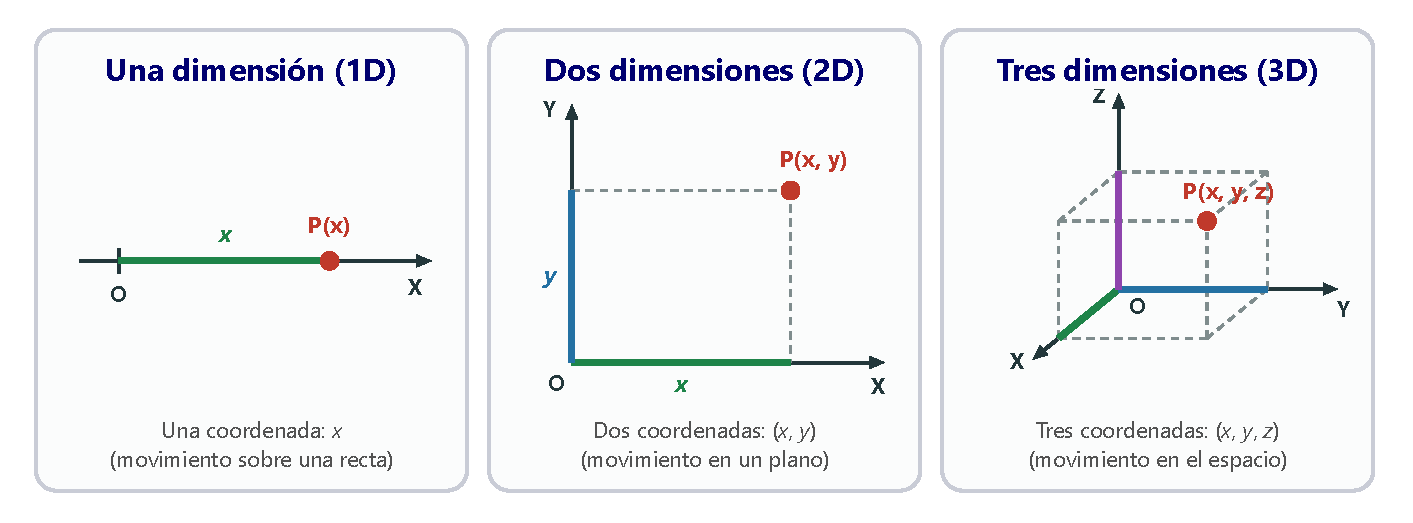
\includegraphics[width=0.95\textwidth]{images/UD8/sistemas_referencia}
    \caption{Según el movimiento, basta con una, dos o tres coordenadas para fijar la posición del móvil.}
    \label{fig:ud8-sr}
\end{figure}

Cualquier sistema de referencia permite describir el movimiento con igual validez, pero unos son más cómodos que otros: para un
coche en una carretera recta basta con un eje (1D); para un balón lanzado a canasta, con un plano (2D); para un avión, con tres
ejes (3D). Lo más práctico suele ser colocar el origen en la \textbf{posición del observador}. Un sistema de referencia siempre está
en reposo respecto a sí mismo, pero puede moverse respecto a otro: por eso se dice que el movimiento es \textbf{relativo}. En el
universo no existe ningún punto en reposo absoluto.

\begin{definition}[Sistemas inerciales y no inerciales]
    Un \textbf{sistema de referencia inercial} es aquel en el que un cuerpo sobre el que no actúa ninguna acción externa está en
    reposo o se mueve en línea recta con velocidad constante. Los sistemas inerciales están en reposo o se mueven con
    \textbf{velocidad constante} unos respecto a otros. Un sistema que tiene \textbf{aceleración} respecto a uno inercial es
    \textbf{no inercial}.
\end{definition}

Volvamos al telesilla. Si se detiene de golpe antes de llegar a la cumbre, la gente que espera en la cola (un S.R. inercial) ve que
tu cuerpo sigue moviéndose hacia delante un instante, porque nada lo ha frenado. Sin embargo, el asiento, que ha frenado
bruscamente, es un S.R. \textbf{no inercial}: desde él parece que algo te ha empujado hacia delante, aunque nadie lo ha hecho.

\begin{remark}
    \textbf{¿Es la Tierra un sistema inercial?} Estrictamente no: gira sobre sí misma y alrededor del Sol, así que tiene
    aceleración. Pero esas aceleraciones son tan pequeñas que, para los movimientos que estudiaremos este curso, la superficie
    terrestre es una \textbf{muy buena aproximación} de un sistema inercial.
\end{remark}

\begin{exercise}
    Indica si los siguientes sistemas se comportan como sistemas de referencia inerciales o no inerciales: a) un tren que arranca
    en la estación; b) un coche que circula a \qty{100}{\km\per\hour} constantes por una autovía recta; c) una niña, quieta en el
    suelo, que observa el vuelo de una cigüeña; d) un ascensor que arranca en la planta baja para subir al quinto piso; e) un
    autobús que toma una rotonda.
    \begin{solu}
        \textcolor{red}{Inerciales: b) y c)}, porque están en reposo o se mueven en línea recta con velocidad constante respecto
        al suelo. \textcolor{red}{No inerciales: a), d) y e)}: el tren y el ascensor aumentan su velocidad, y el autobús cambia la
        dirección de su velocidad; los tres tienen aceleración.
    \end{solu}
\end{exercise}

\subsection{Elementos del movimiento}

Los \textbf{elementos} que describen un movimiento son la \textbf{posición}, la \textbf{trayectoria}, el \textbf{vector
desplazamiento} y el \textbf{espacio recorrido}. Todos ellos dependen del sistema de referencia en que se midan.

\begin{definition}[Posición y trayectoria]
    La \textbf{posición} es el punto del espacio que ocupa el móvil en un instante dado. La \textbf{trayectoria} es el conjunto
    de puntos por los que pasa el móvil a lo largo del tiempo, es decir, la línea que une sus sucesivas posiciones.
\end{definition}

La trayectoria se obtiene registrando las posiciones \(s_0, s_1, s_2\ldots\) que ocupa el móvil en los instantes
\(t_0, t_1, t_2\ldots\) En la práctica, se suele tomar \(t_0 = 0\) al empezar a estudiar el movimiento.

\begin{figure}[H]
    \centering
    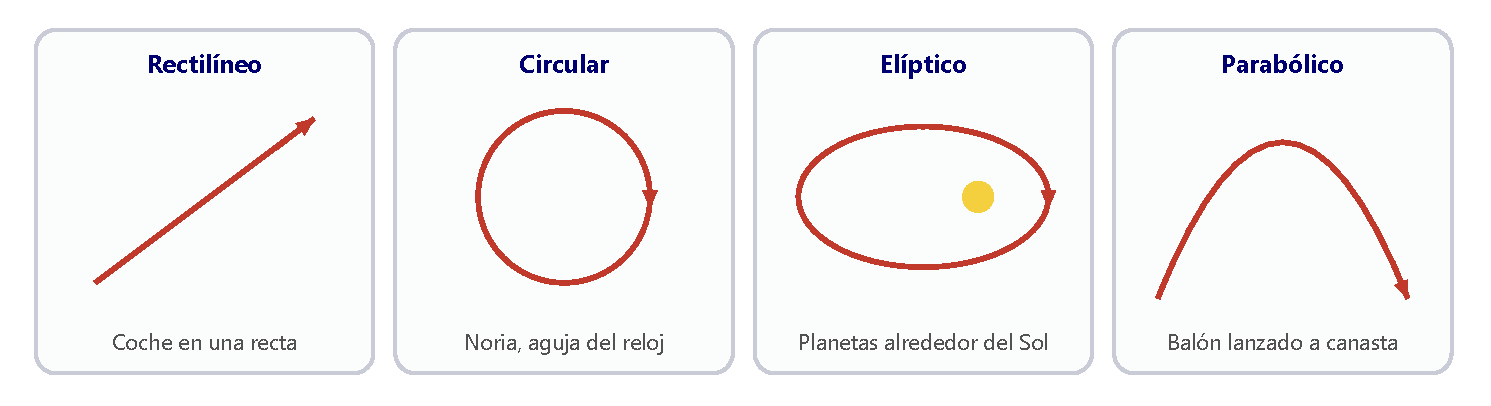
\includegraphics[width=0.85\textwidth]{images/UD8/tipos_trayectoria}
    \caption{Según la forma de la trayectoria, el movimiento es rectilíneo o curvilíneo (circular, elíptico, parabólico\ldots).}
    \label{fig:ud8-tipos}
\end{figure}

%========================================================================================
\section{Descripción del movimiento}\label{sec:ud8-descripcion}
%========================================================================================

\subsection{Vector posición y vector desplazamiento}

En un sistema de referencia de dos dimensiones, con vectores unitarios \(\ivec\) (eje X) y \(\jvec\) (eje Y), las dos magnitudes
básicas para describir el movimiento son vectoriales y se miden en metros:

\begin{definition}[Vector posición]
    El \textbf{vector posición} \(\vec r\) de un móvil es el vector que tiene su origen en el origen O del sistema de referencia
    y su extremo en el punto P\((x, y)\) que ocupa el móvil:
    \[ \vec r = \overrightarrow{OP} = x\,\ivec + y\,\jvec \qquad\qquad |\vec r| = \sqrt{x^2 + y^2} \]
    Su módulo es la distancia del móvil al origen.
\end{definition}

\begin{definition}[Vector desplazamiento]
    El \textbf{vector desplazamiento} \(\Delta\vec r\) es la diferencia entre los vectores posición final e inicial. Va de la
    posición inicial \(P_1(x_1, y_1)\) a la final \(P_2(x_2, y_2)\):
    \[ \Delta\vec r = \vec r_2 - \vec r_1 = (x_2 - x_1)\,\ivec + (y_2 - y_1)\,\jvec = \Delta x\,\ivec + \Delta y\,\jvec
    \qquad\qquad |\Delta\vec r| = \sqrt{(\Delta x)^2 + (\Delta y)^2} \]
\end{definition}

El módulo de un vector se calcula con el \textbf{teorema de Pitágoras} a partir de sus componentes. Si las posiciones inicial y
final coinciden, el desplazamiento es nulo, aunque el cuerpo se haya movido.

\begin{figure}[H]
    \centering
    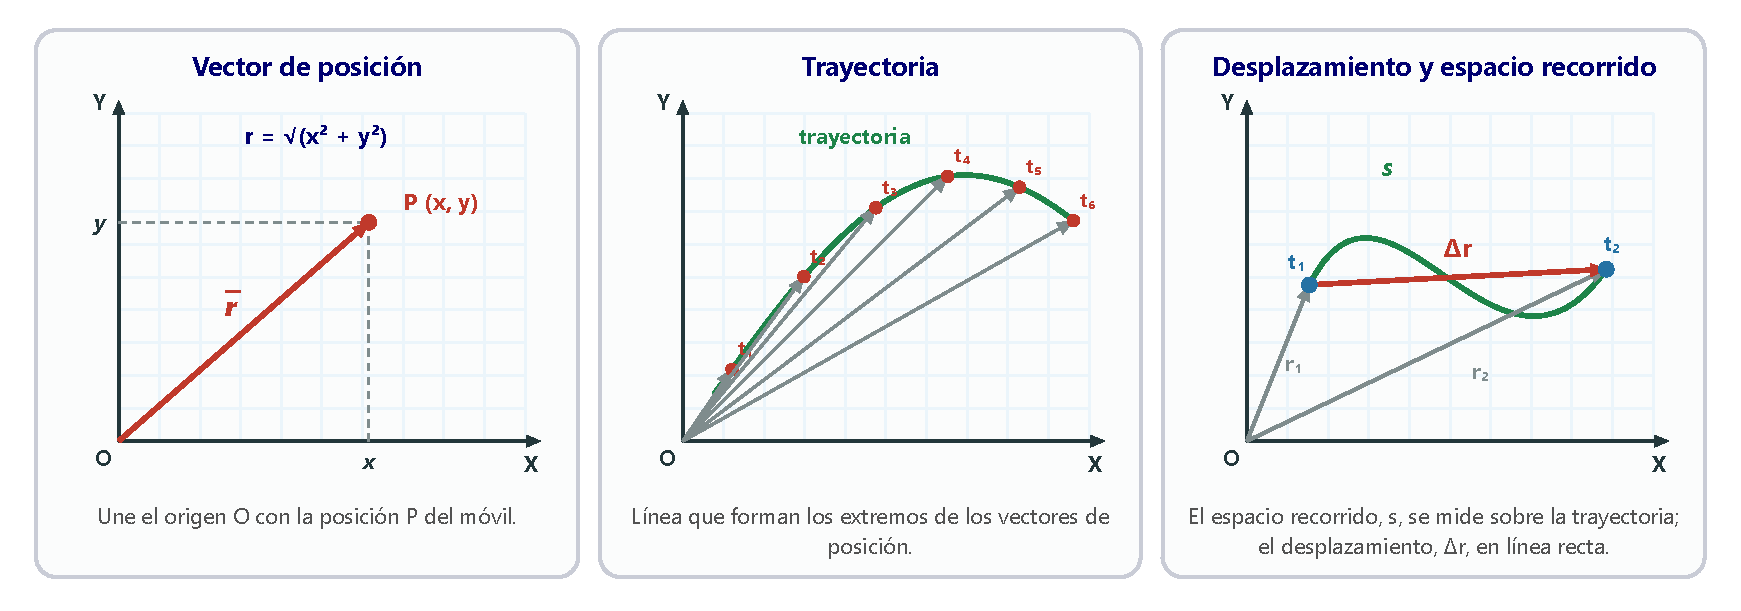
\includegraphics[width=\textwidth]{images/UD8/posicion_trayectoria}
    \caption{Vector posición, trayectoria y diferencia entre el desplazamiento y el espacio recorrido.}
    \label{fig:ud8-posicion}
\end{figure}

\begin{remark}
    \textbf{La posición depende del sistema de referencia.} Si el origen de un segundo sistema, \(O'\), tiene en el primero el
    vector posición \(\overrightarrow{OO'} = x_0\,\ivec + y_0\,\jvec\), la posición del punto P\((x, y)\) para el segundo
    observador es
    \[ \vec r\,' = \vec r - \overrightarrow{OO'} = (x - x_0)\,\ivec + (y - y_0)\,\jvec \]
\end{remark}

\begin{example}
    \textbf{Vectores posición.} Considera los puntos A\((0, 3)\), B\((-2, 0)\) y C\((4, 1)\), con las coordenadas en metros.
    a) Escribe sus vectores posición respecto al origen O\((0, 0)\) y calcula sus módulos. b) Escribe los vectores posición de
    A, B y C para un observador situado en \(O_1(1, 1)\).

    \textbf{Solución.} a) Cada vector posición tiene como componentes las coordenadas del punto:
    \[ \overrightarrow{OA} = 3\,\jvec~\unit{\m} \qquad \overrightarrow{OB} = -2\,\ivec~\unit{\m} \qquad \overrightarrow{OC} = (4\,\ivec + \jvec)~\unit{\m} \]
    \[ |\overrightarrow{OA}| = \qty{3}{\m} \qquad |\overrightarrow{OB}| = \qty{2}{\m} \qquad |\overrightarrow{OC}| = \sqrt{4^2 + 1^2} = \sqrt{17} = \qty{4.12}{\m} \]
    El módulo es la distancia de cada punto al origen: A está \qty{3}{\m} por encima de O; B, \qty{2}{\m} a su izquierda, y C, a
    \qty{4.12}{\m}.

    b) Restamos las coordenadas de \(O_1\):
    \[ \overrightarrow{O_1A} = (0 - 1)\,\ivec + (3 - 1)\,\jvec = (-\ivec + 2\,\jvec)~\unit{\m} \qquad
       \overrightarrow{O_1B} = (-3\,\ivec - \jvec)~\unit{\m} \qquad \overrightarrow{O_1C} = 3\,\ivec~\unit{\m} \]
\end{example}

\begin{example}
    \textbf{Dos caminos.} Una persona juega sobre un tablero de ajedrez gigante como si fuera una pieza; las coordenadas están en
    metros. Parte del punto A\((1, 1)\) y duda entre dos recorridos: ir al punto B\((3, 4)\) y después al C\((5, 7)\), o ir al
    D\((-2, 3)\) y después al E\((-5, 6)\). a) Calcula los vectores desplazamiento de cada tramo y el total de cada recorrido.
    b) ¿Al final de cuál de los dos recorridos queda más cerca de A?

    \textbf{Solución.} a) Primer recorrido:
    \[ \Delta\vec r_{AB} = (3 - 1)\,\ivec + (4 - 1)\,\jvec = (2\,\ivec + 3\,\jvec)~\unit{\m} \qquad
       \Delta\vec r_{BC} = (5 - 3)\,\ivec + (7 - 4)\,\jvec = (2\,\ivec + 3\,\jvec)~\unit{\m} \]
    \[ \Delta\vec r_1 = \Delta\vec r_{AB} + \Delta\vec r_{BC} = (4\,\ivec + 6\,\jvec)~\unit{\m} \]
    Segundo recorrido:
    \[ \Delta\vec r_{AD} = (-3\,\ivec + 2\,\jvec)~\unit{\m} \qquad \Delta\vec r_{DE} = (-3\,\ivec + 3\,\jvec)~\unit{\m} \qquad
       \Delta\vec r_2 = (-6\,\ivec + 5\,\jvec)~\unit{\m} \]
    Observa que el desplazamiento total es la suma de los desplazamientos parciales (y también \(\vec r_C - \vec r_A\)).

    b) \(|\Delta\vec r_1| = \sqrt{4^2 + 6^2} = \sqrt{52} = \qty{7.21}{\m}\) y \(|\Delta\vec r_2| = \sqrt{6^2 + 5^2} = \sqrt{61} =
    \qty{7.81}{\m}\). El punto C está más cerca de A que el punto E.
\end{example}

\begin{exercise}
    El vector posición de un móvil es \(\vec r_1 = (5\,\ivec - 12\,\jvec)~\unit{\m}\). Represéntalo y calcula a qué distancia
    está el móvil del origen.
    \begin{solu}
        \textcolor{blue}{Es una flecha desde O hasta el punto \((5, -12)\).} \(|\vec r_1| = \sqrt{5^2 + 12^2} = \textcolor{red}{\qty{13}{\m}}\).
    \end{solu}
\end{exercise}

\begin{exercise}
    El móvil del ejercicio anterior se desplaza hasta la posición \(\vec r_2 = (-8\,\ivec + 6\,\jvec)~\unit{\m}\). a) Represéntala
    en el mismo gráfico y calcula su módulo. b) Calcula el vector desplazamiento y su módulo, y dibújalo.
    \begin{solu}
        a) \(|\vec r_2| = \sqrt{64 + 36} = \textcolor{red}{\qty{10}{\m}}\). b) \(\Delta\vec r = \vec r_2 - \vec r_1 =
        \textcolor{red}{(-13\,\ivec + 18\,\jvec)~\unit{\m}}\), una flecha que va del extremo de \(\vec r_1\) al de \(\vec r_2\);
        \(|\Delta\vec r| = \sqrt{169 + 324} = \sqrt{493} = \textcolor{red}{\qty{22.2}{\m}}\).
    \end{solu}
\end{exercise}

\subsection{Trayectoria y espacio recorrido}

No hay que confundir dos conceptos que a menudo se mezclan:
\begin{itemize}
    \item la \textbf{trayectoria} es un concepto geométrico: la \textbf{línea} formada por los puntos que va ocupando el móvil;
    no tiene unidades;
    \item el \textbf{espacio recorrido}, \(e\) (o \(\Delta s\)), es la \textbf{distancia medida sobre la trayectoria}; es una
    magnitud \textbf{escalar} y se mide en metros.
\end{itemize}
Tampoco hay que confundir el espacio recorrido con el \textbf{módulo del desplazamiento}, que es la distancia \textbf{en línea
recta} entre la posición inicial y la final.

\begin{remark}
    \textbf{¿Una o dos dimensiones?} Los movimientos rectilíneos se suelen estudiar como unidimensionales, colocando el eje X sobre
    la propia trayectoria. Pero también se pueden describir en dos dimensiones si el origen del sistema de referencia está fuera
    de la recta; en ese caso, la posición tiene dos coordenadas que cambian a la vez.
\end{remark}

\begin{example}
    \textbf{Ida y vuelta.} Lucía sale de casa y camina en línea recta los \qty{300}{\m} que la separan de la biblioteca a
    \qty{1.5}{\m\per\s}. Estudia una hora y vuelve a casa por el mismo camino a \qty{2}{\m\per\s}. a) ¿Cuál ha sido su
    desplazamiento? b) ¿Qué espacio ha recorrido?

    \textbf{Solución.} a) Lucía vuelve al punto de partida: las posiciones inicial y final coinciden, así que
    \(\Delta\vec r = \vec 0\) y su desplazamiento es nulo. b) Ha recorrido \qty{300}{\m} a la ida y \qty{300}{\m} a la vuelta:
    \(e = \qty{600}{\m}\). (Las velocidades no influyen en ninguno de los dos resultados.)
\end{example}

\begin{exercise}
    Dos amigos suben a una atracción de feria en la que una plataforma circular de \qty{4}{\m} de radio da vueltas durante
    \qty{40}{\s}. Si en ese tiempo dan exactamente 6 vueltas, ¿cuál ha sido su desplazamiento y qué espacio han recorrido?
    \begin{solu}
        \textcolor{blue}{Acaban en el mismo punto en que empezaron.} \(\Delta\vec r = \vec 0\): \textcolor{red}{desplazamiento nulo};
        \(e = 6 \cdot 2\pi \cdot 4 = \textcolor{red}{\qty{151}{\m}}\).
    \end{solu}
\end{exercise}

\begin{exercise}
    En una excursión del instituto recorréis \qty{9}{\km} en dirección norte y después \qty{12}{\km} en dirección oeste. Calcula
    el módulo del desplazamiento y el espacio recorrido.
    \begin{solu}
        \textcolor{blue}{Tomando el eje X hacia el este y el Y hacia el norte: \(\Delta\vec r = (-12\,\ivec + 9\,\jvec)~\unit{\km}\).}
        \(|\Delta\vec r| = \sqrt{144 + 81} = \textcolor{red}{\qty{15}{\km}}\); \(e = 9 + 12 = \textcolor{red}{\qty{21}{\km}}\).
    \end{solu}
\end{exercise}

\subsection{El vector posición en función del tiempo}

Para describir completamente un movimiento hay que saber dónde está el móvil en \textbf{cada instante}. Para ello se expresan sus
coordenadas como funciones del tiempo:

\begin{definition}[Ecuación del movimiento]
    La \textbf{ecuación del movimiento} es la expresión del vector posición en función del tiempo:
    \[ \vec r(t) = x(t)\,\ivec + y(t)\,\jvec \]
    Dando valores a \(t\), se obtienen las coordenadas del móvil en ese instante. Las funciones \(x(t)\) e \(y(t)\) se llaman
    \textbf{ecuaciones paramétricas} del movimiento.
\end{definition}

El módulo \(|\vec r(t)| = \sqrt{x(t)^2 + y(t)^2}\) es la distancia del móvil al origen en el instante \(t\).

\subsection{El vector desplazamiento en función del tiempo}

Si \(\Delta t = t_2 - t_1\) es el intervalo de tiempo transcurrido entre dos instantes, el desplazamiento en ese intervalo es
\[ \Delta\vec r = \vec r(t_2) - \vec r(t_1) = (x_2 - x_1)\,\ivec + (y_2 - y_1)\,\jvec \qquad\qquad
   |\Delta\vec r| = \sqrt{(x_2 - x_1)^2 + (y_2 - y_1)^2} \]
En general, \(|\Delta\vec r|\) \textbf{no coincide con el espacio recorrido}, salvo en trayectorias rectilíneas sin cambio de
sentido. En una trayectoria cerrada, \(\Delta\vec r = \vec 0\), pero \(e \neq 0\).

\begin{example}
    \textbf{Movimiento en una dimensión.} La posición de un móvil sobre una recta viene dada por \(x(t) = 4t^2 - 2t\), en unidades
    del SI. Calcula: a) su posición en \(t = 0\), \(t = \qty{3}{\s}\) y \(t = \qty{8}{\s}\); b) su desplazamiento entre los
    segundos 3 y 8.

    \textbf{Solución.} a) Sustituimos cada valor de \(t\) en la ecuación:
    \[ x(0) = 0 \qquad x(3) = 4 \cdot 9 - 2 \cdot 3 = \qty{30}{\m} \qquad x(8) = 4 \cdot 64 - 2 \cdot 8 = \qty{240}{\m} \]
    b) \(\Delta x = x(8) - x(3) = 240 - 30 = \qty{210}{\m}\).
\end{example}

\begin{example}
    \textbf{Movimiento en el plano.} La posición de un móvil varía según \(\vec r(t) = (t^2 - 3t)\,\ivec + (4t + 2)\,\jvec\), en
    unidades del SI. a) Calcula su posición en \(t = 0\), \(t = \qty{2}{\s}\) y \(t = \qty{5}{\s}\). b) Determina el vector
    desplazamiento entre \(t = 0\) y \(t = \qty{2}{\s}\) y entre \(t = 0\) y \(t = \qty{5}{\s}\), y sus módulos.

    \textbf{Solución.} a) \(\vec r(0) = 2\,\jvec~\unit{\m}\); \(\vec r(2) = (4 - 6)\,\ivec + (8 + 2)\,\jvec = (-2\,\ivec + 10\,\jvec)~\unit{\m}\);
    \(\vec r(5) = (25 - 15)\,\ivec + (20 + 2)\,\jvec = (10\,\ivec + 22\,\jvec)~\unit{\m}\).

    b) \(\Delta\vec r_{0,2} = (-2\,\ivec + 10\,\jvec) - 2\,\jvec = (-2\,\ivec + 8\,\jvec)~\unit{\m}\), con módulo
    \(\sqrt{4 + 64} = \qty{8.25}{\m}\). \(\Delta\vec r_{0,5} = (10\,\ivec + 20\,\jvec)~\unit{\m}\), con módulo
    \(\sqrt{100 + 400} = \qty{22.4}{\m}\): el móvil está a \qty{8.25}{\m} de su punto de partida a los \qty{2}{\s}, y a
    \qty{22.4}{\m} a los \qty{5}{\s}.
\end{example}

\begin{example}
    \textbf{En una pista de skate.} Una rampa de skate tiene forma de media circunferencia de \qty{2.5}{\m} de radio. Calcula el
    desplazamiento y el espacio recorrido por un patinador que va: a) desde el borde de un lado (A) hasta el borde del otro lado
    (F); b) desde el borde A hasta el punto más bajo (M).

    \textbf{Solución.} El desplazamiento se mide en línea recta y el espacio, sobre el arco de circunferencia.
    a) A y F están en los extremos de un diámetro: \(|\Delta\vec r_{AF}| = 2r = \qty{5}{\m}\). El arco es media circunferencia:
    \(e_{AF} = \pi r = \qty{7.85}{\m}\).
    b) A y M forman un ángulo recto con el centro: \(|\Delta\vec r_{AM}| = \sqrt{r^2 + r^2} = r\sqrt 2 = \qty{3.54}{\m}\). El arco es
    un cuarto de circunferencia: \(e_{AM} = \dfrac{2\pi r}{4} = \qty{3.93}{\m}\). En las trayectorias curvas, el desplazamiento y
    el espacio recorrido no coinciden.
\end{example}

\begin{exercise}
    El vector posición de una cometa viene dado por \(\vec r(t) = 3t\,\ivec - (4t^2 + 2)\,\jvec\), en unidades del SI.
    a) Calcula su posición en \(t = 0\), \(t = \qty{4}{\s}\) y \(t = \qty{8}{\s}\). b) Determina el vector desplazamiento entre
    \(t = 0\) y \(t = \qty{4}{\s}\) y entre \(t = 0\) y \(t = \qty{8}{\s}\). c) Calcula sus módulos e interpreta el resultado.
    \begin{solu}
        a) \(\textcolor{red}{\vec r(0) = -2\,\jvec~\unit{\m}}\); \(\textcolor{red}{\vec r(4) = (12\,\ivec - 66\,\jvec)~\unit{\m}}\);
        \(\textcolor{red}{\vec r(8) = (24\,\ivec - 258\,\jvec)~\unit{\m}}\). b) \(\textcolor{red}{\Delta\vec r_{0,4} = (12\,\ivec - 64\,\jvec)~\unit{\m}}\);
        \(\textcolor{red}{\Delta\vec r_{0,8} = (24\,\ivec - 256\,\jvec)~\unit{\m}}\). c) \(\textcolor{red}{\qty{65.1}{\m}}\) y
        \(\textcolor{red}{\qty{257}{\m}}\): son las distancias en línea recta entre la posición inicial y las posiciones a los 4 y
        a los \qty{8}{\s}. (Con estos datos, la cometa estaría cayendo cada vez más deprisa: el eje Y apunta hacia arriba.)
    \end{solu}
\end{exercise}

\begin{exercise}
    La posición de un pez viene dada por \(\vec r(t) = 3t\,\ivec + (2t - 4)\,\jvec\), en unidades del SI. a) Calcula el
    desplazamiento del pez durante los seis primeros segundos. b) Calcula el desplazamiento durante los tres últimos segundos de
    ese intervalo e interpreta el resultado.
    \begin{solu}
        a) \(\vec r(0) = -4\,\jvec\); \(\vec r(6) = 18\,\ivec + 8\,\jvec\); \(\Delta\vec r = \textcolor{red}{(18\,\ivec + 12\,\jvec)~\unit{\m}}\).
        b) \(\vec r(3) = 9\,\ivec + 2\,\jvec\); \(\Delta\vec r = \textcolor{red}{(9\,\ivec + 6\,\jvec)~\unit{\m}}\): es la mitad
        del anterior en la mitad de tiempo, porque las coordenadas son funciones de primer grado de \(t\): el pez se mueve en
        línea recta y recorre lo mismo en cada segundo.
    \end{solu}
\end{exercise}

\subsection{La ecuación de la trayectoria}

Las ecuaciones paramétricas \(x(t)\) e \(y(t)\) están relacionadas a través del tiempo. Si eliminamos \(t\) entre ellas, obtenemos
una relación directa entre las coordenadas:

\begin{definition}[Ecuación de la trayectoria]
    La \textbf{ecuación de la trayectoria} se obtiene despejando \(t\) en una de las ecuaciones paramétricas y sustituyéndolo en la
    otra. Queda de la forma \(y = f(x)\) o \(x = f(y)\), y su gráfica es la forma de la trayectoria.
\end{definition}

Si la ecuación de la trayectoria es de primer grado, la trayectoria es una \textbf{recta}; si es de segundo grado, por ejemplo
\(y = a x^2 + b x + c\), es una \textbf{parábola}; y en general las funciones de grado superior dan trayectorias curvas.

\begin{example}
    \textbf{Trayectoria rectilínea.} Calcula la ecuación de la trayectoria de un móvil cuyo vector posición es
    \(\vec r(t) = (2t + 1)\,\ivec + (3t - 2)\,\jvec\), en metros, y represéntala.

    \textbf{Solución.} Separamos las coordenadas: \(x = 2t + 1\) e \(y = 3t - 2\). Despejamos \(t\) de la primera,
    \(t = \dfrac{x - 1}{2}\), y lo sustituimos en la segunda:
    \[ y = 3 \cdot \frac{x - 1}{2} - 2 \quad\Rightarrow\quad y = \frac{3x - 7}{2} \]
    Es una función de primer grado: la trayectoria es una \textbf{recta} (figura~\ref{fig:ud8-trayectorias}, izquierda).
\end{example}

\begin{example}
    \textbf{Trayectoria parabólica.} En los vuelos de entrenamiento en ingravidez, el avión describe una parábola. Determina la
    ecuación de la trayectoria de un avión de este tipo a partir de su vector posición, \(\vec r(t) = 8t\,\ivec + (2 - 5t^2)\,\jvec\)
    (en hectómetros y segundos), y represéntala.

    \textbf{Solución.} \(x = 8t\) e \(y = 2 - 5t^2\). Despejamos \(t = \dfrac{x}{8}\) y sustituimos:
    \[ y = 2 - 5 \left(\frac{x}{8}\right)^2 \quad\Rightarrow\quad y = 2 - \frac{5}{64}\,x^2 \]
    Es una función de segundo grado: la trayectoria es una \textbf{parábola} (figura~\ref{fig:ud8-trayectorias}, derecha). Solo
    tiene sentido físico para \(t \geq 0\), es decir, para \(x \geq 0\).
\end{example}

\begin{figure}[H]
    \centering
    \begin{tikzpicture}
        \begin{axis}[grafica, axis lines=middle, xlabel={\(x\) (m)}, ylabel={\(y\) (m)}, xmin=-1, xmax=7, ymin=-4, ymax=8,
            every axis x label/.style={at={(ticklabel* cs:1)}, anchor=west},
            every axis y label/.style={at={(ticklabel* cs:1)}, anchor=south}]
            \addplot[very thick, ocre, domain=1:7] {(3*x - 7)/2};
            \addplot[only marks, mark=*, mark size=1.8pt, ocre] coordinates {(1,-2) (3,1) (5,4) (7,7)};
            \node[font=\scriptsize, anchor=west] at (axis cs:3.1,0.6) {\(t = \qty{1}{\s}\)};
            \node[font=\scriptsize, anchor=west] at (axis cs:1.1,-2.6) {\(t = 0\)};
        \end{axis}
    \end{tikzpicture}\hspace{1cm}
    \begin{tikzpicture}
        \begin{axis}[grafica, axis lines=middle, xlabel={\(x\) (hm)}, ylabel={\(y\) (hm)}, xmin=-0.5, xmax=6, ymin=-1, ymax=2.6,
            every axis x label/.style={at={(ticklabel* cs:1)}, anchor=west},
            every axis y label/.style={at={(ticklabel* cs:1)}, anchor=south}]
            \addplot[very thick, ocre, domain=0:5.5] {2 - 5*x^2/64};
            \addplot[only marks, mark=*, mark size=1.8pt, ocre] coordinates {(0,2) (4,0.75)};
            \node[font=\scriptsize, anchor=south west] at (axis cs:0.1,2) {\(t = 0\)};
            \node[font=\scriptsize, anchor=south west] at (axis cs:4,0.8) {\(t = \qty{0.5}{\s}\)};
        \end{axis}
    \end{tikzpicture}
    \caption{Trayectorias de los ejemplos: una recta, \(y = (3x - 7)/2\), y una parábola, \(y = 2 - 5x^2/64\).}
    \label{fig:ud8-trayectorias}
\end{figure}

\begin{exercise}
    Un móvil se mueve según la ecuación \(\vec r(t) = (t + 5)\,\ivec + (3 - 6t)\,\jvec\), en metros. Determina analítica y
    gráficamente la ecuación de su trayectoria.
    \begin{solu}
        \textcolor{blue}{\(t = x - 5\); \(y = 3 - 6(x - 5)\).} \(\textcolor{red}{y = -6x + 33}\): una recta de pendiente \(-6\) que
        corta al eje Y en 33 (el móvil empieza en el punto \((5, 3)\)).
    \end{solu}
\end{exercise}

\begin{exercise}
    Calcula la ecuación de la trayectoria de un móvil cuyo vector posición es \(\vec r(t) = (3t - 2)\,\ivec + t^2\,\jvec\), en
    metros, y represéntala.
    \begin{solu}
        \textcolor{blue}{\(t = \dfrac{x + 2}{3}\).} \(\textcolor{red}{y = \dfrac{(x + 2)^2}{9}}\): una parábola con el vértice en
        \((-2, 0)\), que es la posición inicial.
    \end{solu}
\end{exercise}

\begin{exercise}
    El vector \(\vec r(t) = t^3\,\ivec + (5t - 4)\,\jvec\) (en metros) expresa la posición de una cometa durante su vuelo.
    Determina la ecuación de su trayectoria y descríbela.
    \begin{solu}
        \textcolor{blue}{Es más fácil despejar \(t\) de la coordenada \(y\): \(t = \dfrac{y + 4}{5}\).}
        \(\textcolor{red}{x = \left(\dfrac{y + 4}{5}\right)^3}\): es una función de tercer grado, así que la trayectoria es
        \textcolor{red}{curva}.
    \end{solu}
\end{exercise}

%========================================================================================
\section{La velocidad}\label{sec:ud8-velocidad}
%========================================================================================

En el día a día decimos que un vehículo es más rápido que otro si tarda menos en recorrer el mismo tramo. El concepto de velocidad
formaliza esta idea.

\begin{definition}[Velocidad]
    La \textbf{velocidad} es una magnitud física que informa del \textbf{cambio de posición} de un cuerpo y del \textbf{tiempo}
    empleado en él. Su unidad en el SI es el \unit{\m\per\s}.
\end{definition}

Según tengamos en cuenta o no la dirección y el sentido del movimiento, y según la duración del intervalo de tiempo, se definen
varios conceptos de velocidad.

\subsection{La velocidad media}

\begin{definition}[Velocidad media y celeridad media]
    La \textbf{velocidad media} \(\vec v_m\) es el cociente entre el vector desplazamiento y el tiempo empleado en él; es una
    magnitud \textbf{vectorial} con la misma dirección y sentido que \(\Delta\vec r\). La \textbf{celeridad} o \textbf{rapidez
    media} \(v_m\) es el cociente entre el espacio recorrido y el tiempo empleado; es una magnitud \textbf{escalar}:
    \[ \vec v_m = \frac{\Delta\vec r}{\Delta t} \qquad\qquad v_m = \frac{e}{\Delta t} \]
\end{definition}

La rapidez media no es, en general, el módulo de la velocidad media: solo coinciden en un movimiento rectilíneo sin cambios de
sentido. En una trayectoria cerrada, la velocidad media es nula, pero la rapidez media no. El inconveniente de los valores medios es
que no informan de lo que ocurre dentro del intervalo: la rapidez media de un esquiador en un slalom gigante puede ser de unos
\qty{70}{\km\per\hour}, pero no es la misma en la salida, al atravesar las puertas o al llegar a la meta.

\begin{example}
    \textbf{Al parque de atracciones.} Para ir a un parque de atracciones que está a \qty{21}{\km}, un grupo de amigos va en
    bicicleta y tarda \qty{45}{\minute}; otro va en coche y tarda \qty{20}{\minute}. Calcula la rapidez media de cada grupo en el SI.

    \textbf{Solución.} Bicicleta: \(v_{m1} = \dfrac{e}{\Delta t_1} = \dfrac{\qty{21000}{\m}}{45 \cdot \qty{60}{\s}} = \qty{7.78}{\m\per\s}\)
    (\qty{28}{\km\per\hour}). Coche: \(v_{m2} = \dfrac{\qty{21000}{\m}}{20 \cdot \qty{60}{\s}} = \qty{17.5}{\m\per\s}\)
    (\qty{63}{\km\per\hour}).
\end{example}

\begin{exercise}
    En una carrera solidaria, una corredora mantiene una rapidez media de \qty{12}{\km\per\hour} durante \qty{40}{\minute}.
    ¿Qué distancia recorre?
    \begin{solu}
        \(e = v_m\,\Delta t = 12 \cdot \dfrac{40}{60} = \qty{8}{\km} = \textcolor{red}{\qty{8e3}{\m}}\).
    \end{solu}
\end{exercise}

\begin{exercise}
    En un viaje de Sevilla a Madrid conducen dos personas por turnos. La primera recorre \qty{230}{\km} a una rapidez media de
    \qty{115}{\km\per\hour}, y la segunda, los \qty{300}{\km} restantes a \qty{100}{\km\per\hour}. ¿Cuánto dura el viaje? ¿Cuál es
    la rapidez media de todo el viaje?
    \begin{solu}
        \(t_1 = \dfrac{230}{115} = \qty{2}{\hour}\); \(t_2 = \dfrac{300}{100} = \qty{3}{\hour}\); \(\textcolor{red}{t = \qty{5}{\hour}}\).
        \(v_m = \dfrac{530}{5} = \textcolor{red}{\qty{106}{\km\per\hour}}\) (no es la media de las dos rapideces).
    \end{solu}
\end{exercise}

\subsection{La velocidad instantánea}

Cuanto más corto sea el intervalo de tiempo en que calculamos la velocidad media, más precisa será la información sobre el
movimiento. Así surge el concepto de \textbf{velocidad instantánea}, la velocidad que tiene el móvil en un instante concreto.

\begin{definition}[Velocidad instantánea]
    La \textbf{velocidad instantánea} es el límite de la velocidad media cuando el intervalo de tiempo tiende a cero:
    \[ \vec v = \lim_{\Delta t \to 0} \frac{\Delta\vec r}{\Delta t} = \lim_{\Delta t \to 0} \frac{\vec r(t + \Delta t) - \vec r(t)}{\Delta t} \]
\end{definition}

Cuando el intervalo es muy pequeño, el módulo del desplazamiento se confunde con el espacio recorrido, por lo que el módulo de la
velocidad instantánea es la \textbf{rapidez} o \textbf{celeridad instantánea}:
\[ |\vec v| = \lim_{\Delta t \to 0} \frac{|\Delta\vec r|}{\Delta t} = \lim_{\Delta t \to 0} \frac{e}{\Delta t} \]
Es lo que marca el \textbf{velocímetro} de un coche.

\begin{figure}[H]
    \centering
    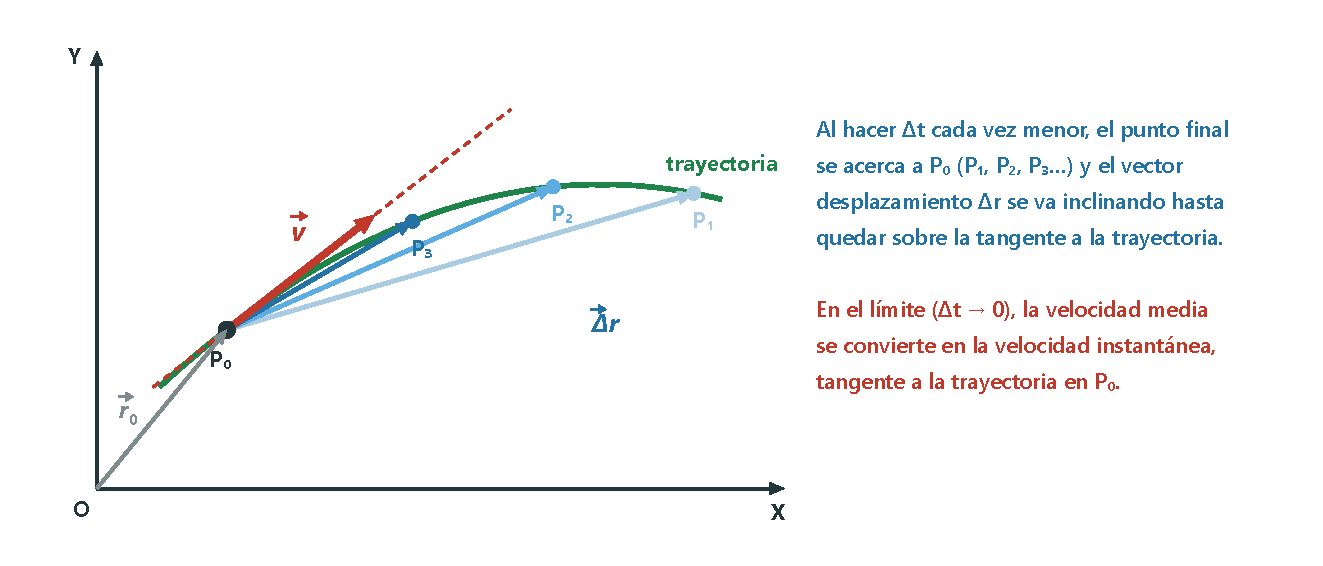
\includegraphics[width=0.85\textwidth]{images/UD8/velocidad_limite}
    \caption{Al reducir el intervalo de tiempo, el desplazamiento tiende a la dirección de la tangente.}
    \label{fig:ud8-limite}
\end{figure}

\begin{example}
    \textbf{Velocidad instantánea con la definición.} El vector posición de un móvil es \(\vec r(t) = 4t\,\ivec + (8 - t^2)\,\jvec\),
    en unidades del SI. a) Halla la velocidad instantánea aplicando la definición. b) Calcula la velocidad en \(t = \qty{1}{\s}\)
    y en \(t = \qty{3}{\s}\).

    \textbf{Solución.} a) Calculamos \(\vec r(t + \Delta t) = 4(t + \Delta t)\,\ivec + \big(8 - (t + \Delta t)^2\big)\,\jvec\) y
    restamos \(\vec r(t)\):
    \[ \vec r(t + \Delta t) - \vec r(t) = 4\,\Delta t\,\ivec + \big(-2t\,\Delta t - (\Delta t)^2\big)\,\jvec \]
    \[ \vec v = \lim_{\Delta t \to 0} \frac{4\,\Delta t\,\ivec + (-2t\,\Delta t - \Delta t^2)\,\jvec}{\Delta t}
       = \lim_{\Delta t \to 0} \big(4\,\ivec + (-2t - \Delta t)\,\jvec\big) = (4\,\ivec - 2t\,\jvec)~\unit{\m\per\s} \]
    b) \(\vec v(1) = (4\,\ivec - 2\,\jvec)~\unit{\m\per\s}\); \(\vec v(3) = (4\,\ivec - 6\,\jvec)~\unit{\m\per\s}\).
\end{example}

\subsubsection{Velocidad instantánea y derivada}

Calcular límites puede ser laborioso. Por suerte, el límite que define la velocidad es una operación matemática muy conocida: la
\textbf{derivada}.

\begin{definition}[Derivada]
    La \textbf{derivada} de una función \(f(t)\) respecto del tiempo indica \textbf{cómo cambia} la función al transcurrir el
    tiempo:
    \[ \frac{\dif f}{\dif t} = \lim_{\Delta t \to 0} \frac{f(t + \Delta t) - f(t)}{\Delta t} \]
    Por tanto, la \textbf{velocidad instantánea es la derivada del vector posición respecto del tiempo}:
    \[ \vec v = \frac{\dif\vec r}{\dif t} \]
\end{definition}

Las derivadas de las funciones más usadas están tabuladas, así que no hace falta calcular el límite cada vez:

\begin{table}[H]
    \centering
    \caption{Derivadas elementales (\(k\) y \(n\) son constantes; \(f\) y \(g\), funciones de \(t\))}
    \vspace{-5pt}
    \begin{tabular}{@{}lclc@{}}
        \toprule
        \textbf{Función} & \textbf{Derivada} & \textbf{Función} & \textbf{Derivada} \\
        \midrule
        \(k\) & \(0\) & \(\sen t\) & \(\cos t\) \\[3pt]
        \(t^n\) & \(n\,t^{n - 1}\) & \(\cos t\) & \(-\sen t\) \\[3pt]
        \(k \cdot f\) & \(k \cdot \dfrac{\dif f}{\dif t}\) & \(e^t\) & \(e^t\) \\[8pt]
        \(f \pm g\) & \(\dfrac{\dif f}{\dif t} \pm \dfrac{\dif g}{\dif t}\) & \(\ln t\) & \(\dfrac{1}{t}\) \\[8pt]
        \(f \cdot g\) & \(\dfrac{\dif f}{\dif t}\,g + f\,\dfrac{\dif g}{\dif t}\) & \(f^n\) & \(n\,f^{n - 1}\,\dfrac{\dif f}{\dif t}\) \\[8pt]
        \(\sen(\omega t)\) & \(\omega\cos(\omega t)\) & \(\sqrt f\) & \(\dfrac{1}{2\sqrt f}\,\dfrac{\dif f}{\dif t}\) \\
        \bottomrule
    \end{tabular}
    \label{tab:ud8-derivadas}
\end{table}

\begin{example}
    \textbf{Con la derivada.} La posición de un balón que rueda por el suelo es \(x(t) = 3 + 6t^2\), en unidades del SI.
    Calcula: a) la expresión de su velocidad; b) su velocidad en \(t = \qty{2}{\s}\) y en \(t = \qty{4}{\s}\).

    \textbf{Solución.} a) \(v(t) = \dfrac{\dif x}{\dif t} = 0 + 6 \cdot 2t = 12t~\unit{\m\per\s}\).
    b) \(v(2) = 12 \cdot 2 = \qty{24}{\m\per\s}\); \(v(4) = 12 \cdot 4 = \qty{48}{\m\per\s}\).
\end{example}

\subsubsection{El vector velocidad instantánea}

En un movimiento en el plano, \(\vec r = x(t)\,\ivec + y(t)\,\jvec\), la velocidad instantánea se obtiene derivando cada
componente por separado:
\[ \vec v = \frac{\dif x}{\dif t}\,\ivec + \frac{\dif y}{\dif t}\,\jvec = v_x\,\ivec + v_y\,\jvec \]
Las derivadas de las coordenadas son las componentes \(v_x\) y \(v_y\) de la velocidad. El vector velocidad instantánea tiene:
\begin{itemize}
    \item \textbf{módulo}: la rapidez del móvil, \(|\vec v| = \sqrt{v_x^2 + v_y^2}\);
    \item \textbf{dirección}: la de la recta \textbf{tangente} a la trayectoria en cada punto;
    \item \textbf{sentido}: el del movimiento.
\end{itemize}

\begin{figure}[H]
    \centering
    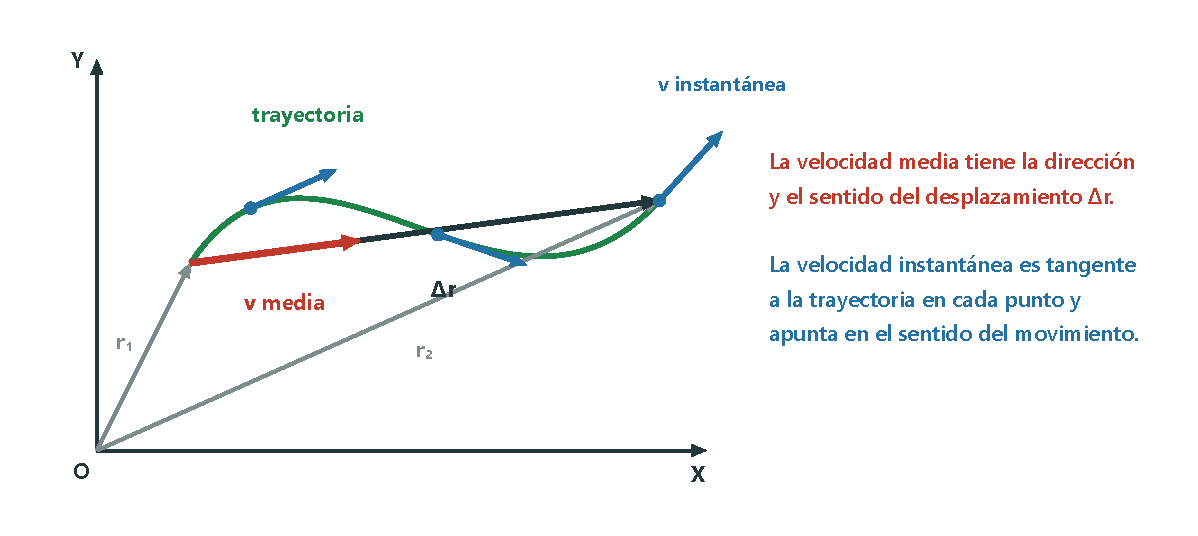
\includegraphics[width=0.8\textwidth]{images/UD8/velocidad_vector}
    \caption{La velocidad media tiene la dirección del desplazamiento; la instantánea es tangente a la trayectoria.}
    \label{fig:ud8-velocidad}
\end{figure}

\begin{example}
    \textbf{Vector velocidad y rapidez.} A partir de \(\vec r(t) = (0{,}5\,t^2 + 2)\,\ivec + (0{,}2\,t^2 - 1)\,\jvec\), en unidades
    del SI, determina: a) el vector velocidad instantánea; b) la velocidad en \(t = \qty{5}{\s}\); c) la rapidez en ese instante.

    \textbf{Solución.} a) Derivamos cada componente: \(\vec v(t) = 0{,}5 \cdot 2t\,\ivec + 0{,}2 \cdot 2t\,\jvec =
    (t\,\ivec + 0{,}4\,t\,\jvec)~\unit{\m\per\s}\). b) \(\vec v(5) = (5\,\ivec + 2\,\jvec)~\unit{\m\per\s}\).
    c) \(|\vec v(5)| = \sqrt{5^2 + 2^2} = \sqrt{29} = \qty{5.39}{\m\per\s}\).
\end{example}

\begin{exercise}
    El vector posición de una atracción de feria es \(\vec r(t) = (2t^2 + 1)\,\ivec + 3t\,\jvec\), en metros. Calcula: a) la
    expresión de la velocidad instantánea; b) el vector velocidad en \(t = \qty{2}{\s}\) y en \(t = \qty{4}{\s}\).
    \begin{solu}
        a) \(\textcolor{red}{\vec v = (4t\,\ivec + 3\,\jvec)~\unit{\m\per\s}}\). b) \(\textcolor{red}{\vec v(2) = (8\,\ivec + 3\,\jvec)~\unit{\m\per\s}}\);
        \(\textcolor{red}{\vec v(4) = (16\,\ivec + 3\,\jvec)~\unit{\m\per\s}}\).
    \end{solu}
\end{exercise}

\begin{exercise}
    Un coche teledirigido se mueve según \(\vec r(t) = (4t - t^2)\,\ivec + (t^2 - 2)\,\jvec\), en metros. Calcula: a) el módulo de
    la velocidad media en los cinco primeros segundos; b) la rapidez en \(t = \qty{2}{\s}\) y en \(t = \qty{5}{\s}\).
    \begin{solu}
        a) \textcolor{blue}{\(\vec r(0) = -2\,\jvec\); \(\vec r(5) = -5\,\ivec + 23\,\jvec\); \(\Delta\vec r = -5\,\ivec + 25\,\jvec\);
        \(\vec v_m = -\ivec + 5\,\jvec\).} \(|\vec v_m| = \sqrt{26} = \textcolor{red}{\qty{5.10}{\m\per\s}}\).
        b) \textcolor{blue}{\(\vec v = (4 - 2t)\,\ivec + 2t\,\jvec\).} \(\vec v(2) = 4\,\jvec\): \(\textcolor{red}{\qty{4}{\m\per\s}}\);
        \(\vec v(5) = -6\,\ivec + 10\,\jvec\): \(\sqrt{136} = \textcolor{red}{\qty{11.7}{\m\per\s}}\).
    \end{solu}
\end{exercise}

\subsection{La velocidad es relativa}

La posición y la trayectoria dependen del sistema de referencia, y también la velocidad: es una magnitud \textbf{relativa}.
Supongamos que dos observadores, O y A, miden la posición de un mismo cuerpo B. El observador O ve a A en la posición
\(\vec r_{AO}\) y a B en \(\vec r_{BO}\); el observador A ve a B en \(\vec r_{BA}\). Como se ve en la figura, \(\vec r_{BO} =
\vec r_{AO} + \vec r_{BA}\). Derivando respecto del tiempo:
\[ \vec v_{BO} = \vec v_{AO} + \vec v_{BA} \quad\Rightarrow\quad \boxed{\vec v_{BA} = \vec v_{BO} - \vec v_{AO}} \]
\(\vec v_{BA}\) es la \textbf{velocidad relativa} de B respecto a A. Esta relación entre las velocidades que miden dos observadores
inerciales es la \textbf{transformación de velocidades de Galileo}.

\begin{figure}[H]
    \centering
    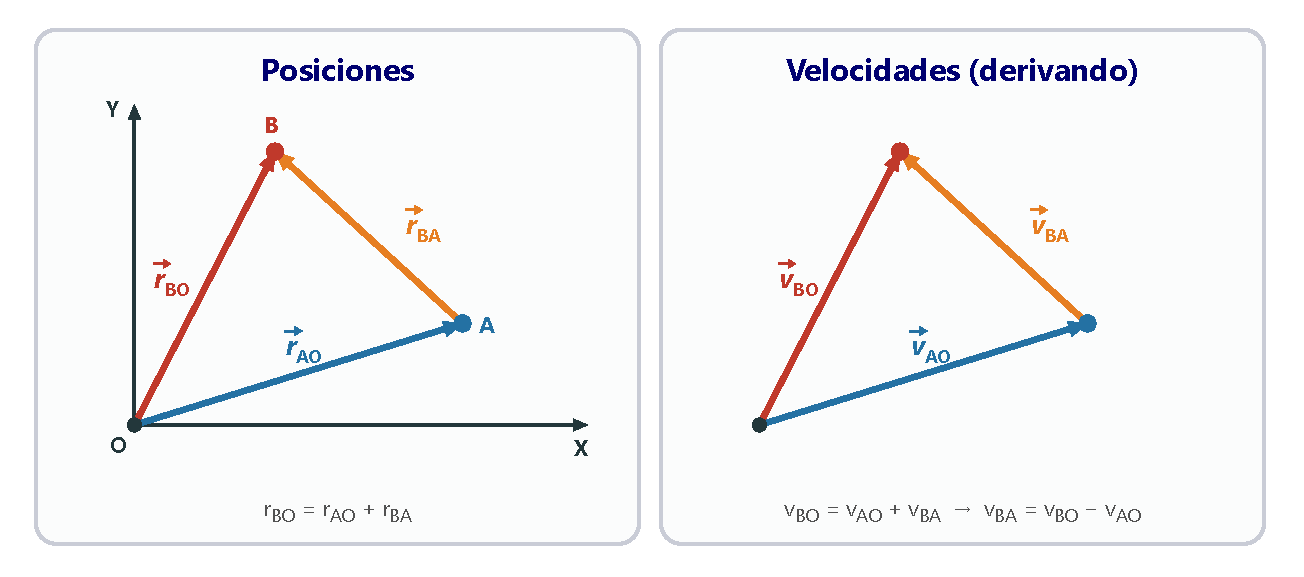
\includegraphics[width=0.75\textwidth]{images/UD8/velocidad_relativa}
    \caption{Posiciones y velocidades de un cuerpo B medidas por dos observadores, O y A.}
    \label{fig:ud8-relativa}
\end{figure}

\begin{remark}
    \textbf{Transformación de aceleraciones.} Si derivamos de nuevo, \(\vec a_{BO} = \vec a_{AO} + \vec a_{BA}\). Cuando los dos
    observadores son inerciales, A se mueve respecto a O con velocidad constante, así que \(\vec a_{AO} = \vec 0\) y queda
    \(\vec a_{BO} = \vec a_{BA}\): \textbf{todos los observadores inerciales miden la misma aceleración} para un cuerpo, aunque
    midan velocidades distintas.
\end{remark}

\begin{example}
    \textbf{En la carretera.} Por una carretera recta circulan un coche a \qty{90}{\km\per\hour} y una moto a \qty{110}{\km\per\hour}
    en el mismo sentido, y un camión a \qty{80}{\km\per\hour} en sentido contrario. Calcula la velocidad de la moto, del camión y
    del propio conductor del coche medidas desde el coche.

    \textbf{Solución.} Tomamos el eje X en el sentido del coche. Respecto al suelo: \(\vec v_C = 90\,\ivec\), \(\vec v_M = 110\,\ivec\)
    y \(\vec v_K = -80\,\ivec\) (en \unit{\km\per\hour}). El sistema de referencia es el coche:
    \[ \vec v_{M\text{-}C} = \vec v_M - \vec v_C = 110\,\ivec - 90\,\ivec = 20\,\ivec~\unit{\km\per\hour} \qquad
       \vec v_{K\text{-}C} = -80\,\ivec - 90\,\ivec = -170\,\ivec~\unit{\km\per\hour} \]
    El conductor se mueve con el coche: su velocidad relativa es nula. Por eso el camión parece «venir muy deprisa» y la moto
    nos adelanta despacio.
\end{example}

\begin{exercise}
    Un tren pasa por el andén a \qty{5}{\m\per\s}. Un viajero que va a perderlo corre tras él a \qty{7}{\m\per\s}, y dentro del
    tren el revisor camina hacia la cabina a \qty{1.5}{\m\per\s} respecto al tren. Determina: a) la velocidad del viajero
    respecto al tren; b) la velocidad del revisor respecto a la estación.
    \begin{solu}
        a) \(v_{VT} = 7 - 5 = \textcolor{red}{\qty{2}{\m\per\s}}\) en el sentido del tren: le alcanza. b) \(v_{RE} = 5 + \num{1.5} =
        \textcolor{red}{\qty{6.5}{\m\per\s}}\).
    \end{solu}
\end{exercise}

%========================================================================================
\section{La aceleración}\label{sec:ud8-aceleracion}
%========================================================================================

Si un cuerpo está sometido a interacciones, su velocidad puede cambiar en cualquiera de sus características: el
\textbf{módulo}, la \textbf{dirección} o el \textbf{sentido}. Un saltador de esquí aumenta su rapidez sin cambiar de dirección; un
\textit{snowboarder} cambia la dirección de su velocidad en cada giro; un yoyó cambia de sentido casi sin cambiar de rapidez.

\begin{definition}[Aceleración]
    La \textbf{aceleración} es una magnitud vectorial que mide los \textbf{cambios} que sufre el \textbf{vector velocidad} a lo
    largo del tiempo, ya sea en módulo, en dirección o en sentido. Su unidad en el SI es el \unit{\m\per\s\squared}.
\end{definition}

Siempre que la velocidad cambie, aunque sea mínimamente, la aceleración será distinta de cero. Según el tipo de cambio, hablaremos de
\textbf{aceleración tangencial} o de \textbf{aceleración normal} (o centrípeta), las componentes intrínsecas de la aceleración.

\subsection{La aceleración media}

\begin{definition}[Aceleración media]
    La \textbf{aceleración media} \(\vec a_m\) relaciona el cambio del vector velocidad con el intervalo de tiempo transcurrido:
    \[ \vec a_m = \frac{\Delta\vec v}{\Delta t} = \frac{\vec v_2 - \vec v_1}{t_2 - t_1} \]
    Tiene la misma dirección y sentido que el vector \(\Delta\vec v\).
\end{definition}

\begin{figure}[H]
    \centering
    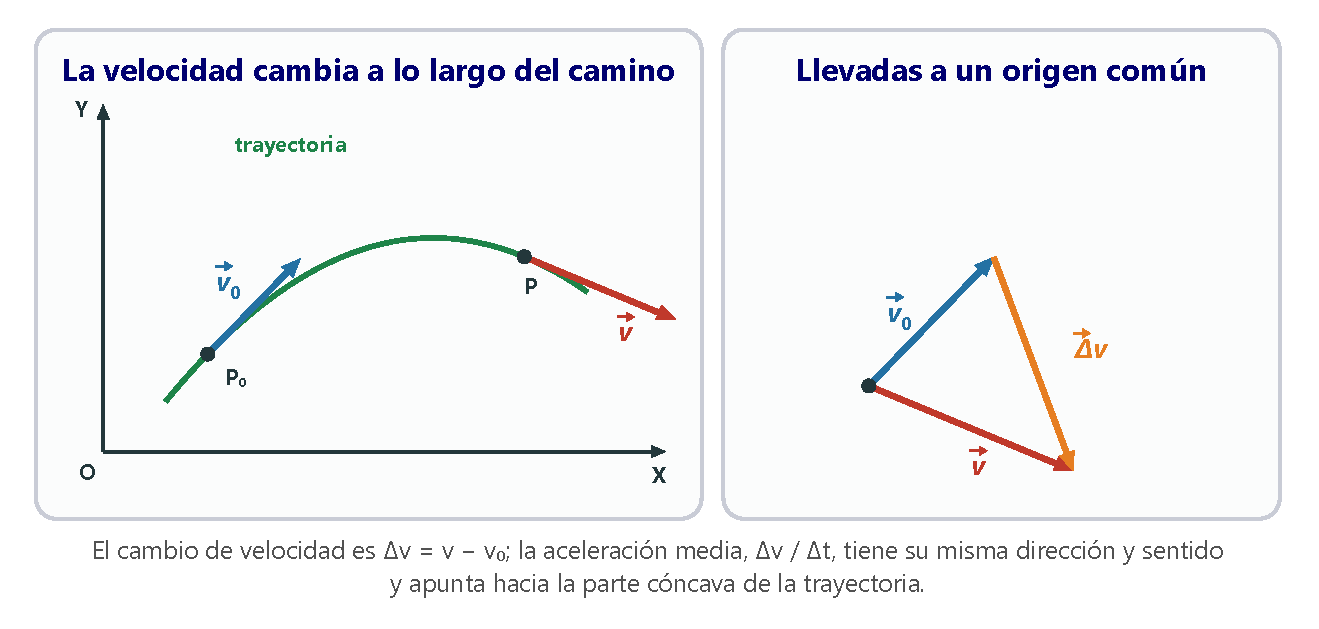
\includegraphics[width=0.85\textwidth]{images/UD8/aceleracion_media}
    \caption{En una trayectoria curva, \(\Delta\vec v\) (y la aceleración media) apunta hacia el interior de la curva.}
    \label{fig:ud8-am}
\end{figure}

\subsection{La aceleración instantánea}

\begin{definition}[Aceleración instantánea]
    La \textbf{aceleración instantánea} es el límite de la aceleración media cuando el intervalo de tiempo tiende a cero, es decir,
    la \textbf{derivada de la velocidad respecto del tiempo}:
    \[ \vec a = \lim_{\Delta t \to 0} \frac{\Delta\vec v}{\Delta t} = \frac{\dif\vec v}{\dif t} \]
\end{definition}

En el plano, si \(\vec v = v_x(t)\,\ivec + v_y(t)\,\jvec\), se deriva cada componente:
\[ \vec a = \frac{\dif v_x}{\dif t}\,\ivec + \frac{\dif v_y}{\dif t}\,\jvec = a_x\,\ivec + a_y\,\jvec \qquad\qquad |\vec a| = \sqrt{a_x^2 + a_y^2} \]
Como la velocidad es la derivada de la posición, la aceleración se obtiene derivando \textbf{dos veces} el vector posición:
\(\vec a = \dfrac{\dif^2\vec r}{\dif t^2}\).

La aceleración instantánea tiene la dirección y el sentido de \(\dif\vec v\), que en general \textbf{no es tangente} a la
trayectoria. En los movimientos rectilíneos tiene la dirección de la velocidad, aunque su sentido puede ser el mismo (el móvil
acelera) o el contrario (frena).

\begin{example}
    \textbf{Velocidad y aceleración en una dimensión.} Un objeto se mueve según \(x(t) = t^3 - 4t^2 + 2\), en unidades del SI.
    Determina: a) la expresión de la velocidad; b) la de la aceleración; c) la velocidad en \(t = \qty{4}{\s}\) y en
    \(t = \qty{6}{\s}\); d) la aceleración media entre esos instantes; e) la aceleración instantánea en \(t = \qty{4}{\s}\).

    \textbf{Solución.} a) \(v(t) = \dfrac{\dif x}{\dif t} = (3t^2 - 8t)~\unit{\m\per\s}\). b) \(a(t) = \dfrac{\dif v}{\dif t} =
    (6t - 8)~\unit{\m\per\s\squared}\). c) \(v(4) = 48 - 32 = \qty{16}{\m\per\s}\); \(v(6) = 108 - 48 = \qty{60}{\m\per\s}\).
    d) \(a_m = \dfrac{60 - 16}{6 - 4} = \qty{22}{\m\per\s\squared}\). e) \(a(4) = 24 - 8 = \qty{16}{\m\per\s\squared}\).
    La aceleración no es constante, así que la media y la instantánea son distintas.
\end{example}

\begin{example}
    \textbf{Aceleración media en el plano.} Un móvil tiene una velocidad \(\vec v(t) = -2t^2\,\ivec + 6\,\jvec\), en unidades del
    SI. Calcula la aceleración media en los cinco primeros segundos.

    \textbf{Solución.} \(\vec v(0) = 6\,\jvec~\unit{\m\per\s}\) y \(\vec v(5) = (-50\,\ivec + 6\,\jvec)~\unit{\m\per\s}\):
    \[ \vec a_m = \frac{\vec v(5) - \vec v(0)}{5 - 0} = \frac{-50\,\ivec}{5} = -10\,\ivec~\unit{\m\per\s\squared} \]
    La componente \(v_y\) no cambia, así que solo hay aceleración en el eje X.
\end{example}

\begin{example}
    \textbf{Aceleración con la definición de límite.} La velocidad de un móvil es \(\vec v(t) = (4t^2 - 2t)\,\ivec~\unit{\m\per\s}\).
    a) Calcula la aceleración instantánea con la definición de límite. b) Calcula la aceleración en \(t = \qty{1}{\s}\) y en
    \(t = \qty{5}{\s}\).

    \textbf{Solución.} a) \(\vec v(t + \Delta t) - \vec v(t) = \big[4(t + \Delta t)^2 - 2(t + \Delta t) - 4t^2 + 2t\big]\,\ivec =
    \big(8t\,\Delta t + 4\,\Delta t^2 - 2\,\Delta t\big)\,\ivec\), así que
    \[ \vec a = \lim_{\Delta t \to 0} \frac{(8t\,\Delta t + 4\,\Delta t^2 - 2\,\Delta t)\,\ivec}{\Delta t} =
       \lim_{\Delta t \to 0} (8t + 4\,\Delta t - 2)\,\ivec = (8t - 2)\,\ivec~\unit{\m\per\s\squared} \]
    b) \(\vec a(1) = 6\,\ivec~\unit{\m\per\s\squared}\); \(\vec a(5) = 38\,\ivec~\unit{\m\per\s\squared}\). (Derivando,
    \(\dfrac{\dif}{\dif t}(4t^2 - 2t) = 8t - 2\): el mismo resultado, mucho más rápido.)
\end{example}

\begin{exercise}
    Un patinador se desplaza según la función \(x(t) = 0{,}2\,t^3 + 2t - 5\), en metros. Determina: a) su velocidad; b) su
    aceleración; c) la velocidad en \(t = \qty{2}{\s}\) y en \(t = \qty{5}{\s}\); d) la aceleración media entre esos instantes;
    e) la aceleración en \(t = \qty{4}{\s}\).
    \begin{solu}
        a) \(\textcolor{red}{v = (0{,}6\,t^2 + 2)~\unit{\m\per\s}}\); b) \(\textcolor{red}{a = 1{,}2\,t~\unit{\m\per\s\squared}}\);
        c) \(\textcolor{red}{v(2) = \qty{4.4}{\m\per\s}}\) y \(\textcolor{red}{v(5) = \qty{17}{\m\per\s}}\);
        d) \(a_m = \dfrac{17 - \num{4.4}}{3} = \textcolor{red}{\qty{4.2}{\m\per\s\squared}}\); e) \(\textcolor{red}{a(4) = \qty{4.8}{\m\per\s\squared}}\).
    \end{solu}
\end{exercise}

\begin{exercise}
    Un coche entra en la autovía a \qty{36}{\km\per\hour} y, dos minutos después, circula a \qty{108}{\km\per\hour}. Calcula su
    aceleración media en unidades del SI.
    \begin{solu}
        \(a_m = \dfrac{30 - 10}{120} = \textcolor{red}{\qty{0.167}{\m\per\s\squared}}\).
    \end{solu}
\end{exercise}

\begin{exercise}
    Un objeto se mueve con una velocidad \(\vec v(t) = (2t^2 - 3t)\,\ivec + (t + 4)\,\jvec\), en \unit{\m\per\s}. a) Halla la
    aceleración instantánea con la definición de límite. Calcula: b) la velocidad al inicio y en \(t = \qty{10}{\s}\); c) la
    aceleración media en ese intervalo; d) la aceleración en \(t = \qty{5}{\s}\) y en \(t = \qty{10}{\s}\).
    \begin{solu}
        a) \textcolor{blue}{\(\Delta v_x = 4t\,\Delta t + 2\,\Delta t^2 - 3\,\Delta t\); \(\Delta v_y = \Delta t\).}
        \(\textcolor{red}{\vec a = (4t - 3)\,\ivec + \jvec~\unit{\m\per\s\squared}}\).
        b) \(\vec v(0) = \textcolor{red}{4\,\jvec~\unit{\m\per\s}}\) y \(\vec v(10) = \textcolor{red}{(170\,\ivec + 14\,\jvec)~\unit{\m\per\s}}\).
        c) \(\vec a_m = \Delta\vec v / \Delta t = \textcolor{red}{(17\,\ivec + \jvec)~\unit{\m\per\s\squared}}\).
        d) \(\vec a(5) = \textcolor{red}{(17\,\ivec + \jvec)~\unit{\m\per\s\squared}}\) y
        \(\vec a(10) = \textcolor{red}{(37\,\ivec + \jvec)~\unit{\m\per\s\squared}}\).
    \end{solu}
\end{exercise}

\subsection{Componentes intrínsecas de la aceleración}

Ya sabemos que hay aceleración no solo cuando cambia el valor de la velocidad, sino también cuando cambia su dirección, aunque la
rapidez sea constante. Para separar los dos efectos, se usa un sistema de referencia ligado a cada punto de la trayectoria, con un
eje \textbf{tangente} y otro \textbf{normal} (perpendicular) a ella. Sus vectores unitarios son \(\vec u_t\), tangente a la
trayectoria en el sentido del movimiento, y \(\vec u_n\), perpendicular a ella y dirigido hacia el centro de la curva.

\begin{definition}[Componentes intrínsecas]
    La aceleración se puede escribir como suma de dos componentes, llamadas \textbf{intrínsecas} porque están ligadas a cada punto
    de la trayectoria:
    \[ \vec a = \vec a_t + \vec a_n = a_t\,\vec u_t + a_n\,\vec u_n \qquad\qquad |\vec a| = \sqrt{a_t^2 + a_n^2} \]
\end{definition}

\begin{figure}[H]
    \centering
    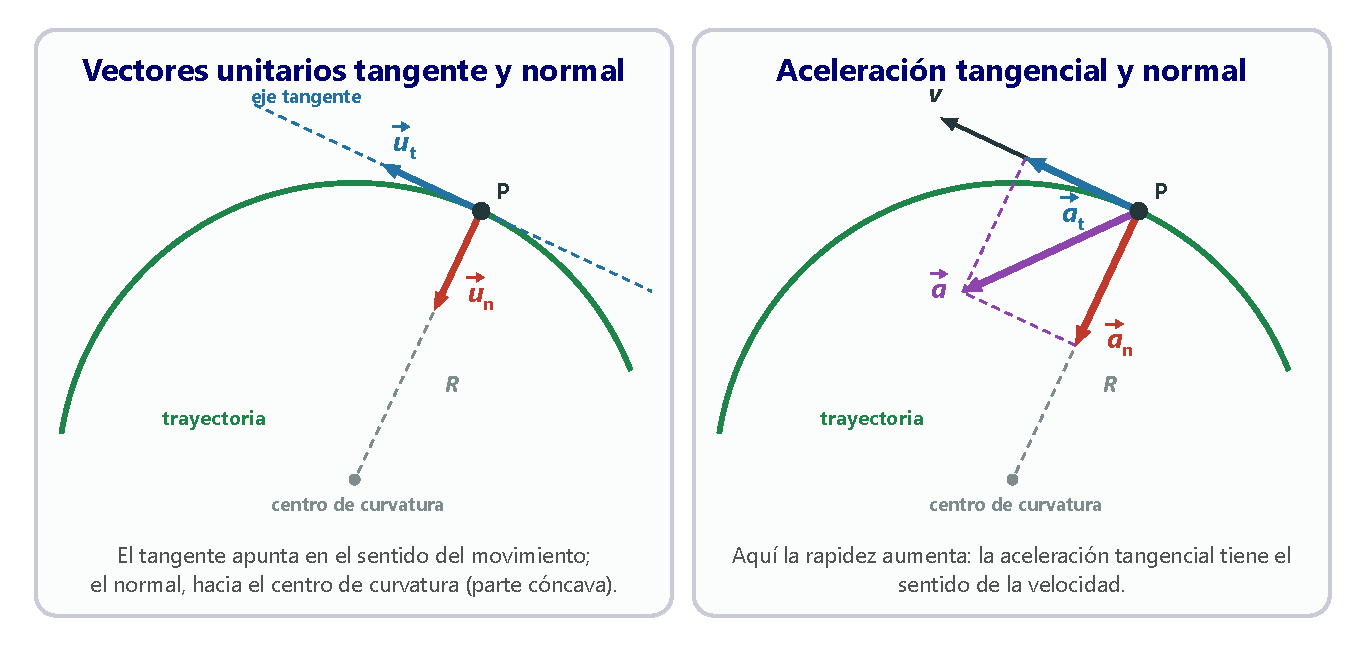
\includegraphics[width=0.9\textwidth]{images/UD8/componentes_intrinsecas}
    \caption{Sistema de referencia intrínseco y componentes tangencial y normal de la aceleración.}
    \label{fig:ud8-intrinsecas}
\end{figure}

\subsubsection{La aceleración tangencial}

Cuando la \textbf{rapidez} de un cuerpo cambia, aparece la \textbf{aceleración tangencial}, \textbf{paralela a la velocidad} en cada
punto. Su valor es la derivada del \textbf{módulo} de la velocidad:
\[ \vec a_t = \frac{\dif |\vec v|}{\dif t}\,\vec u_t \]
Si \(\vec a_t\) tiene el mismo sentido que \(\vec v\), la rapidez aumenta; si tiene sentido contrario, disminuye. Para derivar
el módulo de la velocidad, que suele ser una raíz, son útiles las reglas \(\dfrac{\dif(f^n)}{\dif t} = n\,f^{n - 1}\,\dfrac{\dif f}{\dif t}\)
y \(\dfrac{\dif\sqrt f}{\dif t} = \dfrac{1}{2\sqrt f}\,\dfrac{\dif f}{\dif t}\).

\subsubsection{La aceleración normal o centrípeta}

Cuando la \textbf{dirección} de la velocidad cambia, es decir, en las trayectorias curvas, aparece la \textbf{aceleración normal}
o \textbf{centrípeta}, \textbf{perpendicular a la trayectoria} y dirigida hacia el centro de la curva. Su valor depende de la
rapidez y del radio de curvatura \(R\) en ese punto:
\[ \vec a_n = \frac{v^2}{R}\,\vec u_n \]
En una trayectoria rectilínea, el radio es infinito y \(a_n = 0\). Un móvil puede tener aceleración tangencial, normal, ninguna de
las dos (movimiento rectilíneo y uniforme) o ambas a la vez.

\begin{table}[H]
    \centering
    \caption{Tipos de movimiento según las componentes intrínsecas de la aceleración}
    \vspace{-5pt}
    \begin{tabular}{@{}ccL{8cm}@{}}
        \toprule
        \(\boldsymbol{a_t}\) & \(\boldsymbol{a_n}\) & \textbf{Movimiento} \\
        \midrule
        \(0\) & \(0\) & Rectilíneo uniforme: la velocidad no cambia \\[3pt]
        \(\neq 0\) & \(0\) & Rectilíneo acelerado: cambia solo el módulo de la velocidad \\[3pt]
        \(0\) & \(\neq 0\) & Curvilíneo uniforme (por ejemplo, circular uniforme): cambia solo la dirección \\[3pt]
        \(\neq 0\) & \(\neq 0\) & Curvilíneo acelerado: cambian el módulo y la dirección \\
        \bottomrule
    \end{tabular}
    \label{tab:ud8-intrinsecas}
\end{table}

\begin{example}
    \textbf{Aceleración tangencial y normal a partir del vector posición.} Un cuerpo se mueve según
    \(\vec r(t) = (4t^2 - 1)\,\ivec + 2t^3\,\jvec\), en unidades del SI. Calcula: a) la aceleración tangencial en función del
    tiempo; b) las aceleraciones tangencial, total y normal en \(t = \qty{2}{\s}\); c) el radio de curvatura en ese instante.

    \textbf{Solución.} a) Derivamos para obtener la velocidad y su módulo (para \(t \geq 0\)):
    \[ \vec v = 8t\,\ivec + 6t^2\,\jvec \qquad\qquad |\vec v| = \sqrt{64t^2 + 36t^4} \]
    \[ a_t = \frac{\dif |\vec v|}{\dif t} = \frac{1}{2\sqrt{64t^2 + 36t^4}} \cdot (128t + 144t^3) = \frac{64t + 72t^3}{\sqrt{64t^2 + 36t^4}}~\unit{\m\per\s\squared} \]
    b) \(a_t(2) = \dfrac{128 + 576}{\sqrt{256 + 576}} = \dfrac{704}{\num{28.84}} = \qty{24.4}{\m\per\s\squared}\).
    La aceleración total es \(\vec a = \dfrac{\dif\vec v}{\dif t} = 8\,\ivec + 12t\,\jvec\); en \(t = \qty{2}{\s}\),
    \(\vec a = 8\,\ivec + 24\,\jvec\) y \(|\vec a| = \sqrt{640} = \qty{25.3}{\m\per\s\squared}\). Despejando de
    \(a^2 = a_t^2 + a_n^2\):
    \[ a_n = \sqrt{a^2 - a_t^2} = \sqrt{640 - \num{24.4}^2} = \qty{6.66}{\m\per\s\squared} \]
    c) \(R = \dfrac{v^2}{a_n} = \dfrac{832}{\num{6.66}} = \qty{125}{\m}\).
\end{example}

\begin{example}
    \textbf{En una curva.} Un coche entra en una curva de \qty{20}{\m} de radio a \qty{15}{\m\per\s} y sale de ella a
    \qty{25}{\m\per\s}; tarda \qty{4}{\s} en recorrerla. Calcula: a) la aceleración tangencial, suponiendo que es constante; b) la
    aceleración normal a la entrada y a la salida de la curva; c) el módulo de la aceleración total a la entrada.

    \textbf{Solución.} a) \(a_t = \dfrac{\Delta v}{\Delta t} = \dfrac{25 - 15}{4} = \qty{2.5}{\m\per\s\squared}\).
    b) \(a_{n1} = \dfrac{v_1^2}{R} = \dfrac{15^2}{20} = \qty{11.25}{\m\per\s\squared}\); \(a_{n2} = \dfrac{25^2}{20} =
    \qty{31.25}{\m\per\s\squared}\). c) \(a = \sqrt{a_t^2 + a_n^2} = \sqrt{\num{2.5}^2 + \num{11.25}^2} = \qty{11.5}{\m\per\s\squared}\).
\end{example}

\begin{exercise}
    Calcula la aceleración centrípeta de un niño montado en un tiovivo de \qty{4}{\m} de radio que gira con una rapidez constante
    de \qty{3}{\m\per\s}. ¿Tiene aceleración tangencial?
    \begin{solu}
        \(a_n = \dfrac{3^2}{4} = \textcolor{red}{\qty{2.25}{\m\per\s\squared}}\). \textcolor{red}{No tiene aceleración tangencial},
        porque su rapidez no cambia.
    \end{solu}
\end{exercise}

\begin{exercise}
    Un móvil entra en una curva de \qty{8}{\m} de radio a \qty{4}{\m\per\s} con una aceleración tangencial constante de
    \qty{2}{\m\per\s\squared}. Si tarda \qty{3}{\s} en recorrer la curva, calcula: a) la velocidad y la aceleración normal a la
    salida de la curva; b) la aceleración total en ese momento.
    \begin{solu}
        a) \(v = 4 + 2 \cdot 3 = \textcolor{red}{\qty{10}{\m\per\s}}\); \(a_n = \dfrac{100}{8} = \textcolor{red}{\qty{12.5}{\m\per\s\squared}}\).
        b) \(a = \sqrt{2^2 + \num{12.5}^2} = \textcolor{red}{\qty{12.7}{\m\per\s\squared}}\).
    \end{solu}
\end{exercise}

\begin{exercise}
    Un avión de exhibición describe círculos de \qty{50}{\m} de radio con una rapidez \(v(t) = (2t^2 + 10)~\unit{\m\per\s}\).
    Determina: a) las expresiones de la aceleración tangencial y de la normal, y sus valores en \(t = \qty{3}{\s}\); b) el módulo de
    la aceleración en \(t = \qty{3}{\s}\) y en \(t = \qty{5}{\s}\).
    \begin{solu}
        a) \(\textcolor{red}{a_t = 4t~\unit{\m\per\s\squared}}\); \(\textcolor{red}{a_n = \dfrac{(2t^2 + 10)^2}{50}~\unit{\m\per\s\squared}}\).
        En \(t = \qty{3}{\s}\): \(v = \qty{28}{\m\per\s}\), \(\textcolor{red}{a_t = \qty{12}{\m\per\s\squared}}\) y
        \(\textcolor{red}{a_n = \qty{15.7}{\m\per\s\squared}}\). b) \(a(3) = \sqrt{12^2 + \num{15.68}^2} = \textcolor{red}{\qty{19.7}{\m\per\s\squared}}\);
        en \(t = \qty{5}{\s}\): \(v = \qty{60}{\m\per\s}\), \(a_t = 20\), \(a_n = 72\) y \(a = \textcolor{red}{\qty{74.7}{\m\per\s\squared}}\).
    \end{solu}
\end{exercise}

%========================================================================================
\section{Física en la vida: ¿competiciones más justas gracias a la tecnología?}\label{sec:ud8-cronometraje}
%========================================================================================

En las grandes competiciones de atletismo o de natación, las medallas se deciden a veces por centésimas o incluso milésimas de
segundo. ¿Cómo se miden tiempos tan pequeños?

Durante mucho tiempo el cronometraje fue \textbf{manual}: una persona ponía en marcha el cronómetro al oír el disparo de salida y lo
paraba al ver llegar al deportista, así que el tiempo dependía de sus reflejos. En los Juegos Olímpicos de Los Ángeles de 1932 se
usaron ya decenas de cronógrafos de precisión que medían décimas de segundo. Después llegaron las \textbf{células fotoeléctricas},
que detectan el paso del atleta por la meta, y la \textbf{foto finish}, una cámara que fotografía continuamente la línea de llegada
y permite ordenar a los corredores aunque lleguen casi a la vez. En natación se introdujeron \textbf{placas de contacto} que el
nadador pulsa con la mano al tocar la pared, y en la salida, tacos con sensores que detectan las \textbf{salidas nulas} (un atleta
que reacciona en menos de una décima de segundo después del disparo se considera que ha salido antes de tiempo, porque el ser humano
no puede reaccionar tan deprisa).

Hoy los tiempos se miden con una precisión de milésimas, se transmiten al instante y se completan con sensores que registran la
posición y la velocidad de cada deportista en tiempo real. Pero también surgen preguntas: en los Juegos de Pekín de 2008, Michael
Phelps ganó los 100 metros mariposa por \textbf{una centésima}. ¿Es justa una diferencia tan pequeña? ¿Y si las calles de la
piscina no midieran exactamente lo mismo?

\begin{table}[H]
    \centering
    \caption{Final masculina de 100 metros lisos de los Juegos Olímpicos de Tokio (2021)}
    \vspace{-5pt}
    \begin{tabular}{@{}lcccc@{}}
        \toprule
        \textbf{Atleta} & Jacobs & Kerley & De Grasse & Simbine \\
        \midrule
        \textbf{Tiempo (s)} & \num{9.80} & \num{9.84} & \num{9.89} & \num{9.93} \\
        \bottomrule
    \end{tabular}
    \label{tab:ud8-tokio}
\end{table}

\begin{exercise}
    Con los datos de la tabla~\ref{tab:ud8-tokio}: a) calcula la rapidez media de cada atleta; b) suponiendo que Kerley corriera
    siempre a su rapidez media, ¿a qué distancia de la meta estaba cuando Jacobs la cruzó?; c) ¿qué distancia recorre en una
    centésima de segundo un atleta a \qty{10}{\m\per\s}?; d) en la final de Pekín, Phelps hizo \qty{50.58}{\s} en los
    \qty{100}{\m}. ¿Por cuántos centímetros ganó? e) Debatid: ¿ha hecho la tecnología más justas las competiciones? ¿Cómo ha
    cambiado la participación de las mujeres en los Juegos Olímpicos en los últimos cien años?
    \begin{solu}
        a) \(v_m = 100/t\): \textcolor{red}{Jacobs \qty{10.20}{\m\per\s}; Kerley \qty{10.16}{\m\per\s}; De Grasse
        \qty{10.11}{\m\per\s}; Simbine \qty{10.07}{\m\per\s}}. b) En \qty{9.80}{\s}, Kerley recorre
        \(\num{10.163} \cdot \num{9.80} = \qty{99.59}{\m}\): estaba a \(\textcolor{red}{\approx \qty{41}{\cm}}\) de la meta.
        c) \(10 \cdot \num{0.01} = \textcolor{red}{\qty{0.1}{\m} = \qty{10}{\cm}}\). d) \(v_m = \dfrac{100}{\num{50.58}} =
        \qty{1.98}{\m\per\s}\); en \qty{0.01}{\s} recorre \(\textcolor{red}{\approx \qty{2}{\cm}}\). e) \textcolor{red}{Respuesta
        abierta}. En 1900 participaron 22 mujeres entre casi mil deportistas; en Tokio, casi la mitad fueron mujeres.
    \end{solu}
\end{exercise}

%========================================================================================
\section{Prácticas}\label{sec:ud8-practicas}
%========================================================================================

\subsection{Un aerodeslizador casero}

\noindent\begin{minipage}[t]{0.48\textwidth}
    \textbf{Objetivo}
    \begin{itemize}
        \item Construir un aerodeslizador con materiales sencillos, describir su movimiento (trayectoria, desplazamiento y espacio
        recorrido) y medir su rapidez media.
    \end{itemize}
\end{minipage}\hfill
\begin{minipage}[t]{0.48\textwidth}
    \textbf{Material}
    \begin{itemize}
        \item Un CD o DVD viejo, un trozo de cartón, una botella de plástico con tapón de rosca, un globo mediano, pegamento
        termofusible, un punzón, cinta métrica y cronómetro (o el móvil).
    \end{itemize}
\end{minipage}

\medskip
Un \textbf{aerodeslizador} se desplaza sobre un colchón de aire que él mismo expulsa hacia el suelo. Como apenas toca la superficie,
el rozamiento es muy pequeño y se mueve con mucha facilidad. Los de verdad pueden superar los \qty{100}{\km\per\hour} y se usan como
vehículos de rescate, de transporte entre islas o militares.

\begin{figure}[H]
    \centering
    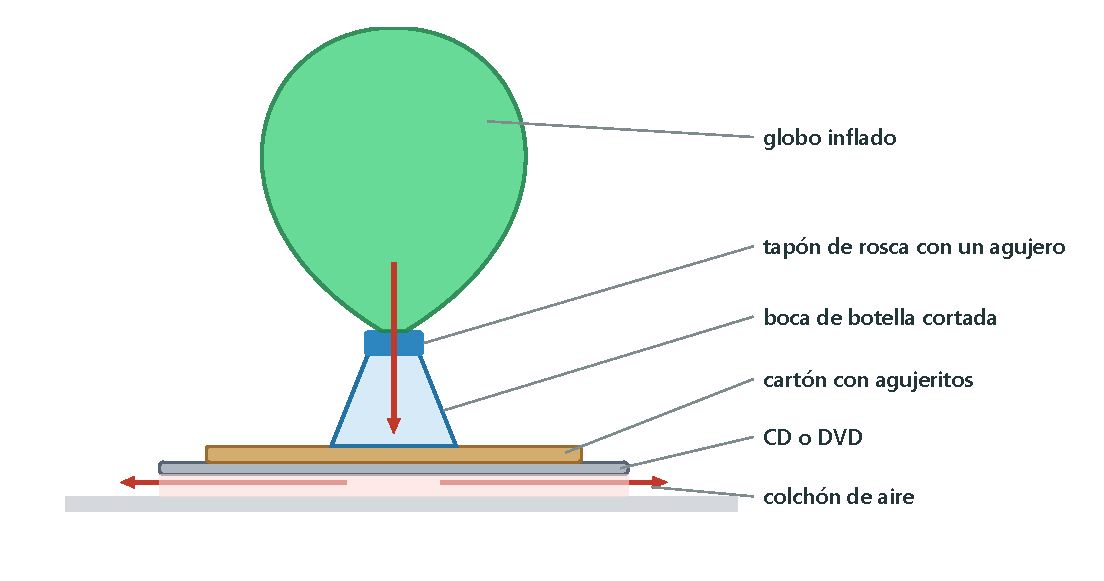
\includegraphics[width=0.55\textwidth]{images/UD8/aerodeslizador}
    \caption{Esquema del aerodeslizador casero: el aire del globo sale por debajo del CD y lo hace flotar.}
    \label{fig:ud8-aerodeslizador}
\end{figure}

\textbf{Procedimiento}
\begin{enumerate}[label=\numberballgreen]
    \item Recorta un círculo de cartón del tamaño del CD (sin el agujero central) y haz con el punzón varios agujeritos en su zona
    central.
    \item Corta la parte superior de la botella, en forma de cono, y haz un agujero de unos \qty{3}{\mm} en el tapón.
    \item Pega el cono de la botella sobre el cartón, tapando los agujeritos, y el cartón sobre el CD, de modo que el aire solo
    pueda salir por el agujero central del disco.
    \item Infla el globo, retuerce la boquilla para que no se escape el aire y encájalo en el tapón.
    \item Coloca el aerodeslizador en una mesa lisa, suelta el globo y dale un pequeño impulso.
    \item Diseña un circuito y mide las distancias recorridas y los tiempos que tarda en recorrerlas. Repite cada medida cinco veces.
    \item Si puedes, graba el movimiento con el móvil y analízalo con un programa de análisis de vídeo, como Tracker.
\end{enumerate}

\begin{exercise}
    a) ¿Por qué el aerodeslizador se mueve con tanta facilidad? ¿Qué ocurre cuando se acaba el aire del globo? b) Describe su
    trayectoria y dibuja el desplazamiento y el espacio recorrido en un recorrido de ida y vuelta. c) En cinco medidas, el
    aerodeslizador tarda 2,3; 2,5; 2,4; 2,6 y \qty{2.2}{\s} en recorrer \qty{1.20}{\m} en línea recta. Calcula el tiempo medio y su
    rapidez media. d) Organiza en una tabla los resultados de tus propias medidas.
    \begin{solu}
        a) \textcolor{red}{Porque el colchón de aire evita casi todo el rozamiento con la mesa}; cuando se acaba el aire, el CD
        toca la mesa y se frena enseguida. b) \textcolor{red}{Respuesta abierta}: en un recorrido de ida y vuelta el desplazamiento
        es nulo y el espacio recorrido es el doble de la distancia. c) \(\bar t = \dfrac{\num{12.0}}{5} = \textcolor{red}{\qty{2.4}{\s}}\);
        \(v_m = \dfrac{\num{1.20}}{\num{2.4}} = \textcolor{red}{\qty{0.50}{\m\per\s}}\). d) \textcolor{red}{Respuesta abierta}.
    \end{solu}
\end{exercise}

\subsection{De la velocidad media a la instantánea con un vídeo}

\noindent\begin{minipage}[t]{0.48\textwidth}
    \textbf{Objetivo}
    \begin{itemize}
        \item Obtener la posición de un móvil en función del tiempo a partir de un vídeo y calcular su velocidad y su aceleración.
    \end{itemize}
\end{minipage}\hfill
\begin{minipage}[t]{0.48\textwidth}
    \textbf{Material}
    \begin{itemize}
        \item Una tabla larga o un carril inclinado, una canica o un coche de juguete, una cinta métrica y un móvil con cámara;
        programa Tracker (gratuito) o una hoja de cálculo.
    \end{itemize}
\end{minipage}

\textbf{Procedimiento}
\begin{enumerate}[label=\numberballgreen]
    \item Inclina ligeramente la tabla y pega a su lado la cinta métrica, que servirá de escala.
    \item Graba con el móvil, fijo y perpendicular a la tabla, cómo baja la canica soltada desde el reposo.
    \item Con Tracker, marca la posición de la canica fotograma a fotograma (o pausa el vídeo cada pocos fotogramas y lee la cinta).
    \item Anota en una tabla las parejas (\(t\), \(x\)) y representa \(x\) frente a \(t\).
\end{enumerate}

\begin{table}[H]
    \centering
    \caption{Posición de una canica que baja por un carril inclinado, obtenida de un vídeo}
    \vspace{-5pt}
    \begin{tabular}{@{}lcccccc@{}}
        \toprule
        \(\boldsymbol{t}\) \textbf{(s)} & 0 & \num{0.2} & \num{0.4} & \num{0.6} & \num{0.8} & \num{1.0} \\
        \midrule
        \(\boldsymbol{x}\) \textbf{(cm)} & 0 & 4 & 16 & 36 & 64 & 100 \\
        \bottomrule
    \end{tabular}
    \label{tab:ud8-canica}
\end{table}

\begin{exercise}
    Con los datos de la tabla~\ref{tab:ud8-canica}: a) calcula la velocidad media en cada intervalo de \qty{0.2}{\s}; b) asigna
    cada velocidad media al instante central de su intervalo y representa \(v\) frente a \(t\). ¿Qué forma tiene la gráfica?
    c) Comprueba que \(x(t) = 100\,t^2\) (en cm y s) y obtén, derivando, \(v(t)\) y \(a(t)\). d) ¿Por qué la velocidad media en un
    intervalo coincide aquí con la instantánea en su punto medio?
    \begin{solu}
        a) \(\textcolor{red}{20, 60, 100, 140~\text{y}~\qty{180}{\cm\per\s}}\). b) En \(t = \numlist{0.1;0.3;0.5;0.7;0.9}~\unit{\s}\):
        los puntos están \textcolor{red}{alineados en una recta que pasa por el origen}, \(v = 200\,t\). c) \(x(0{,}4) = 100 \cdot
        \num{0.16} = 16\) \ldots\ se cumple; \(\textcolor{red}{v = 200\,t~\unit{\cm\per\s}}\) y \(\textcolor{red}{a = \qty{200}{\cm\per\s\squared}
        = \qty{2}{\m\per\s\squared}}\), constante. d) \textcolor{red}{Porque la velocidad cambia de forma lineal con el tiempo}
        (aceleración constante): su valor medio en un intervalo es el valor en el instante central.
    \end{solu}
\end{exercise}

%========================================================================================
\section{Situación de aprendizaje: movilidad sostenible en tu ciudad (ODS 11)}\label{sec:ud8-ods}
%========================================================================================

Más de la mitad de la población mundial vive ya en ciudades, y se calcula que en 2050 lo harán casi siete de cada diez personas. El
\textbf{Objetivo de Desarrollo Sostenible 11} (ciudades y comunidades sostenibles) busca que las ciudades sean inclusivas, seguras,
resilientes y sostenibles. Uno de sus grandes retos es la \textbf{movilidad}: el tráfico es una de las principales fuentes de
contaminación del aire, de ruido y de emisiones de gases de efecto invernadero en las ciudades. Además, los productos que consumimos
recorren cada vez más kilómetros desde donde se producen hasta nuestra mesa: consumir \textbf{productos de proximidad} reduce
también las emisiones del transporte.

\begin{marker}
    \textbf{Reto:} elaborad un \textbf{plan de movilidad sostenible} para llegar al instituto, con datos de vuestra propia clase,
    y presentadlo al resto del centro (o al ayuntamiento).
\end{marker}

\begin{enumerate}[label=\numberballred]
    \item \textbf{Investigad.} ¿Cómo ha cambiado la población de las ciudades y de los pueblos de España en el último siglo? ¿Qué
    tipo de municipios han ganado habitantes y cuáles los han perdido? ¿Cómo afecta esto a la sostenibilidad?
    \item \textbf{Medid.} Haced una encuesta en clase: distancia de casa al instituto, medio de transporte y tiempo que se tarda.
    Calculad la rapidez media de cada medio de transporte.
    \item \textbf{Calculad.} Usad los valores aproximados de la tabla~\ref{tab:ud8-movilidad} para estimar el tiempo de cada
    trayecto con cada medio y las emisiones de \ch{CO2} de toda la clase durante un curso (unos 175 días lectivos, ida y vuelta).
    \item \textbf{Comunicad.} El plan debe incluir: los resultados de la encuesta, los cálculos, un mapa con rutas seguras para ir
    a pie o en bicicleta y propuestas concretas (caminos escolares, aparcabicis, consumo de productos locales\ldots).
\end{enumerate}

\begin{table}[H]
    \centering
    \caption{Rapidez media en ciudad y emisiones aproximadas de \ch{CO2} por persona y kilómetro}
    \vspace{-5pt}
    \begin{tabular}{@{}lcc@{}}
        \toprule
        \textbf{Medio} & \textbf{Rapidez media (km/h)} & \textbf{Emisiones (g de \ch{CO2}/km)} \\
        \midrule
        A pie & 5 & 0 \\[3pt]
        Bicicleta & 15 & 0 \\[3pt]
        Autobús urbano & 18 & 70 \\[3pt]
        Coche (una persona) & 25 & 140 \\
        \bottomrule
    \end{tabular}
    \label{tab:ud8-movilidad}
\end{table}

\begin{exercise}
    Una alumna vive a \qty{2.4}{\km} del instituto. a) ¿Cuánto tarda en llegar a pie, en bicicleta y en coche, según la
    tabla~\ref{tab:ud8-movilidad}? b) ¿Cuánto \ch{CO2} emite en un curso si la llevan en coche (ida y vuelta, 175 días)? c) ¿Por
    qué la rapidez media del coche en la ciudad es tan baja, si puede ir a \qty{50}{\km\per\hour}?
    \begin{solu}
        a) \(t = e / v_m\): \textcolor{red}{a pie, \(\num{2.4}/5 = \qty{0.48}{\hour} \approx \qty{29}{\minute}\); en bicicleta,
        \qty{9.6}{\minute}; en coche, \qty{5.8}{\minute}} (más el tiempo de aparcar). b) \(m = 2 \cdot \num{2.4} \cdot 140 \cdot 175 =
        \qty{117600}{\gram} \approx \textcolor{red}{\qty{118}{\kilo\gram}}\) de \ch{CO2}. c) \textcolor{red}{Porque la rapidez media
        incluye las paradas en semáforos, los atascos y las aceleraciones y frenadas}: el coche pasa mucho tiempo parado.
    \end{solu}
\end{exercise}
